\documentclass[UTF8,a4paper,zihao=-4,openany]{ctexrep}

\usepackage[a4paper,left=2.8cm,right=2.6cm,top=2.6cm,bottom=2.6cm]{geometry}
\usepackage{setspace}
\usepackage{graphicx}
\usepackage{xcolor}
\usepackage{booktabs}
\usepackage{longtable}
\usepackage{array}
\usepackage{tabularx}
\usepackage{multirow}
\usepackage{enumitem}
\usepackage{amsmath,amssymb}
\usepackage{tikz}
\usepackage{pgfplots}
\usepackage{listings}
\usepackage{fancyhdr}
\usepackage{hyperref}
\usepackage{titlesec}
\usepackage{caption}
\usepackage{subcaption}
\usepackage{float}
\usepackage{colortbl}
\usepackage{textcomp}

\pgfplotsset{compat=1.18}
\usetikzlibrary{arrows.meta,positioning,shapes.geometric,calc,fit,backgrounds,shapes.multipart,decorations.pathreplacing}

\hypersetup{
  colorlinks=true,
  linkcolor=black,
  citecolor=black,
  urlcolor=blue,
  pdfauthor={},
  pdftitle={数字遗产管家作品报告}}

\setstretch{1.3}
\setlength{\parindent}{2em}
\setlength{\parskip}{0.1em}
\raggedbottom
\setlist{nosep,leftmargin=2em,itemsep=0pt,topsep=0pt,partopsep=0pt,parsep=0pt}
\captionsetup{font=small,labelfont=bf,justification=centering}

\pagestyle{fancy}

\fancyhf{}
\fancyhead[C]{数字遗产管家作品报告}
\fancyfoot[C]{\thepage}
\renewcommand{\headrulewidth}{0.4pt}

\titleformat{\chapter}{\centering\bfseries\zihao{3}}{第\chinese{chapter}章}{1em}{}
\titleformat{\section}{\bfseries\zihao{4}}{\thesection}{0.8em}{}
\titleformat{\subsection}{\bfseries\zihao{-4}}{\thesubsection}{0.8em}{}

\lstdefinestyle{code}{
  basicstyle=\ttfamily\footnotesize,
  breaklines=true,
  frame=single,
  numbers=left,
  numberstyle=\tiny,
  keywordstyle=\color{blue!70!black},
  commentstyle=\color{green!40!black},
  stringstyle=\color{red!60!black},
  columns=fullflexible,
  keepspaces=true,
  aboveskip=0.5em,
  belowskip=0.5em
}
\lstset{style=code}

\lstdefinestyle{solidity}{
  basicstyle=\ttfamily\footnotesize,
  breaklines=true,
  frame=single,
  numbers=left,
  numberstyle=\tiny,
  keywordstyle=\color{blue!70!black}\bfseries,
  commentstyle=\color{green!40!black},
  stringstyle=\color{red!60!black},
  columns=fullflexible,
  keepspaces=true,
  aboveskip=0.5em,
  belowskip=0.5em,
  keywords={contract,function,uint256,address,bytes32,string,struct,enum,mapping,event,modifier,require,emit,public,view,returns,memory,storage,indexed,if,else,for,bool,true,false,return}
}

% Custom commands
\newcommand{\project}{基于门限密码与同态承诺的数字遗产管家}
\newcommand{\englishname}{Digital Legacy Guardian: Verifiable Digital Asset Inheritance based on Threshold Cryptography}
\newcommand{\riskline}[3]{#1 & #2 & #3\\}
\newcommand{\apiline}[3]{#1 & #2 & #3\\}

\newcommand{\ReviewCard}[5]{
\clearpage
\subsection{#1}
\begin{table}[H]
\centering
\caption{#1专项分析}
\begin{tabularx}{\textwidth}{>{\bfseries}p{3.1cm}X}
\toprule
分析对象 & #2\\
安全目标 & #3\\
实现依据 & #4\\
验证方式 & #5\\
\bottomrule
\end{tabularx}
\end{table}
\noindent
#2是系统在“托管、触发、恢复”生命周期中的一个关键控制点。本作品将该控制点拆解为输入约束、状态约束、密码学约束和审计约束四类条件，确保任何单一角色、单一服务或单一份额都不能独立越过继承门限。

从实现角度看，#4。报告将该实现与前端交互、后端接口、存储结构和智能合约状态机统一建模，使其既能用于竞赛演示，也能作为后续工程化迭代的检查清单。

在测试角度，#5。测试重点不是只证明”正常流程可走通”，而是覆盖篡改份额、重复提交、时间锁未到期、监护人身份不匹配、接口参数缺失等逆向路径，验证系统在异常情况下能够失败在正确位置。
}

\begin{document}
\zihao{-4}
\songti

% ==================== TITLE PAGE ====================
\begin{titlepage}
\centering
\vspace*{2.2cm}
{\zihao{2}\bfseries 2025年全国大学生信息安全竞赛\par}
\vspace{1.2cm}
{\zihao{1}\bfseries 作品报告\par}
\vspace{2.4cm}
\begin{tabular}{rl}
作品名称：& \project\\[0.8cm]
电子邮箱：& \underline{\hspace{8cm}}\\[0.8cm]
提交日期：& \underline{\hspace{8cm}}\\
\end{tabular}
\vfill
\end{titlepage}

% ==================== 摘要 ====================
\chapter*{摘要}
\addcontentsline{toc}{chapter}{摘要}

加密货币私钥、云端账户、加密文件和智能合约权限等数字资产已成为新型个人财产。据统计，全球加密货币持有者超4.2亿人，因私钥丢失永久无法访问的比特币达370余万枚。传统遗嘱、公证和平台申诉机制在数字资产场景中面临困境：私钥无法通过法院强制转移，提前公开凭据带来泄露风险，中心化平台恢复流程周期长且覆盖范围有限。本作品\project（\englishname）围绕数字遗产继承问题，设计并实现了一个基于门限密码学、可验证秘密共享和智能合约的数字资产继承系统。

系统采用 React + TypeScript 前端、Node.js + Express 后端和 Solidity 智能合约三层架构，将数字遗产继承抽象为”资产托管、条件触发、份额验证、密钥恢复、资产释放”五个有序阶段，每个阶段设密码学和状态双重约束。核心安全机制包括：在 secp256k1 标量域上实现 Shamir Secret Sharing，主密钥拆分为 $n$ 个份额，任意 $t$ 个可通过拉格朗日插值恢复，少于 $t$ 个从信息论角度无法推断秘密；引入双多项式 Pedersen 同态承诺结构，实现 server 零信任的可验证份额分发与同态刷新；在份额验证层面，构建了两层互补的密码学验证机制——Pedersen 单点承诺验证（$C_i = r_iG + v_iH$）在提交时即阻止份额值篡改，主承诺同态聚合验证（$\sum \lambda_i C_i = C_{\text{master}}$）确保一组份额来源于原始秘密共享实例，双层验证使伪造份额在提交阶段即被密码学强度拒绝；采用 StoredShare 与 Share 差分设计，持久化仅存承诺值和盲因子，份额明文在邮件分发后丢弃，服务器不保存可恢复密钥的敏感数据。资产经 AES-256 加密存储，加密密钥即为被门限拆分的秘密，形成加密层与门限层双层防护。

在工程层面，前端提供四步向导、控制台面板、监护人门户和 AI 助手，降低门限密码学参数配置门槛。后端实现 PBKDF2 认证、邮件通知、继承管理和资产恢复服务链路。智能合约定义三态状态机和三种触发模式。测试覆盖 26 个核心用例，验证了伪造份额拒绝、未达门限恢复失败和时间锁触发拦截等逆向安全场景。本作品将数字遗产继承从理论转化为可运行的全栈原型，兼顾密码学安全强度与用户操作便利性，可服务于加密资产持有人、数字创作者、跨地域家庭和企业密钥托管等场景。

\textbf{关键词：}数字遗产；门限密码学；Shamir秘密共享；Pedersen承诺；同态刷新；智能合约；抗胁迫

% ==================== 目录 ====================
\setcounter{tocdepth}{1}
\tableofcontents

% ==================== 第一章 作品概述 ====================
\chapter{作品概述}

\section{研究背景}

随着数字经济和区块链技术的快速发展，越来越多的重要资产以数字形式存在。根据 Chainalysis 2024年报告，全球加密货币持有者已超过4.2亿人，仅比特币的市值就曾突破1万亿美元。与此同时，云端存储账户、社交媒体账号、数字版权作品、NFT以及智能合约控制权限等数字资产形态不断涌现。与传统实物资产不同，这些数字资产通常依赖密码、私钥或访问令牌进行控制，一旦持有人发生意外、长期失联或失去操作能力，相关资产可能永久无法访问。

传统遗产继承主要依赖法律文书、公证机构和平台申诉机制完成资产交接。然而这些方式在数字资产场景中面临多重困境：首先，私钥和助记词的本质是不可伪造的随机字符串，无法像实物财产那样通过法院判决强制转移；其次，如果持有人提前向第三方公开密码或助记词，会带来持续性的泄露风险；再次，中心化平台的“账户恢复”流程往往需要身份证明、死亡证明等材料，处理周期长且用户体验差；最后，如果完全由持有人独自掌握所有凭据，持有人本身就成为整个资产体系的单点失效点。

对于这一问题，学术界和工业界已经展开了相关研究。Shamir于1979年提出的秘密共享方案为门限恢复提供了理论基础，Feldman于1987年提出的可验证秘密共享增强了方案在敌手模型下的安全性。在工业实践方面，以太坊的社交恢复钱包、Chainlink的去中心化预言机、以及各类密钥管理服务（KMS）也从不同角度探索了密钥托管与恢复的可行方案。

然而，现有方案往往侧重于单一维度的安全性，未将资产托管、条件触发、份额验证、密钥恢复和资产释放等环节整合为统一的生命周期模型。数字遗产继承不仅是一个密码学问题，更是一个涉及安全工程、用户体验和社会规则的复杂系统工程。

针对上述挑战，本作品设计并实现了一套面向数字遗产场景的安全继承系统。系统利用门限密码学将主密钥拆分为多个份额，由不同监护人分别保管；只有达到预设门限后才能恢复资产访问能力。同时结合可验证秘密共享以及智能合约状态约束机制，实现数字资产从托管、触发到恢复的全生命周期安全管理。

\section{需求分析}

数字遗产继承系统需要同时满足安全性、可用性和可审计性要求。经过对场景的深入分析，本作品总结出以下核心需求：

\textbf{继承可达性需求。}当资产持有人失能、失联或离世后，合法继承人能够在满足预设条件后恢复资产访问权限。系统必须具备明确的触发条件和可靠的恢复流程，使得继承过程不因持有人无法参与而中断。同时，持有人本人在正常状态下仍能自由管理和更新遗产计划。

\textbf{隐私保护需求。}在继承条件触发之前，任何单一监护人、服务器或第三方机构都不能获取完整资产信息。具体而言：第一，服务器存储的计划数据中不应包含份额明文值；第二，单个监护人所持有的份额不足以恢复主密钥；第三，加密资产包的密钥本身也被门限拆分，攻击者必须同时获得密文和足够份额才能解密资产。

\textbf{抗单点失效需求。}系统不能依赖单个用户、单个设备或单个服务节点保存核心秘密。即使部分监护人失联、拒绝配合或恶意操作，只要满足门限数量的诚实监护人参与，系统仍能完成恢复。同时，系统的后端服务本身也不应成为新的单点失效源——即使服务器数据库被读取，攻击者也无法获得主密钥或份额明文。

\textbf{份额真实性需求。}提交的恢复份额必须能够被验证，防止恶意用户提交伪造数据干扰恢复过程。验证机制应具有密码学强度，而非仅依赖格式校验。具体来说，系统必须能够验证：份额值是否与创建时的 Pedersen 承诺匹配；一组份额是否确实来源于原始秘密共享多项式实例。由于盲因子 $r_i$ 存储于服务端，攻击者仅截获公开承诺 $C_i$ 而不知盲因子，无法构造能通过验证的提交。

\textbf{审计追踪需求。}系统应能够记录计划创建、继承申请、份额提交和资产恢复等关键操作，为后续审计提供依据。审计日志应包含操作时间、操作者身份、操作类型和操作结果，但不记录敏感数据（如份额明文值或主密钥）。

\textbf{可用性需求。}系统的用户界面应降低门限密码学参数配置的专业门槛。资产持有人无需理解Shamir多项式的数学原理即可创建遗产计划；监护人只需简单的复制粘贴操作即可提交份额；继承人可以通过清晰的操作指引完成继承流程。

\textbf{兼容性需求。}系统应支持多种数字资产类型，包括但不限于加密货币私钥、云存储账号、加密文件和智能合约权限，并提供统一的资产元数据描述格式。

\section{项目目标}

项目目标可以从功能目标、安全目标和工程目标三个维度进行分解。下表给出了详细的目标说明：

\setlength{\extrarowheight}{4pt}
\begin{longtable}{p{3cm}p{11.4cm}}
\caption{项目目标分解}\\
\toprule
目标类型 & 具体说明\\
\midrule
\endfirsthead
\toprule
目标类型 & 具体说明\\
\midrule
\endhead
功能目标 & 支持用户注册与登录（含验证码机制）；支持创建遗产计划并配置资产、监护人、门限和触发条件；\ 支持发起继承请求并进入份额收集状态；支持监护人提交份额并完成密码学验证；\ 支持达到门限后自动恢复主密钥并解密资产；支持AI助手通过自然语言引导用户完成操作。\\
安全目标 & 主密钥不在任何持久化存储中以明文形式存在；份额明文仅在创建时发送给监护人，不在计划存储中持久化；\ 提交份额前必须通过 Pedersen 单点承诺验证和主承诺同态聚合验证；少于门限数量的份额无法恢复主密钥；\ 加密资产包使用AES加密，密钥即是被门限拆分的秘密。\\
工程目标 & 前后端分离架构，接口清晰，代码分层明确；密码学模块独立封装，可单独测试和迁移；\ 智能合约表达链上状态约束，事件驱动状态转换；项目文档和报告完整，满足竞赛评审要求。\\
展示目标 & 支持从创建计划到继承完成的端到端演示，并能展示篡改份额失败、未达门限恢复失败、\ 时间锁未到期触发失败等多种安全场景。演示过程能够清晰体现密码学验证机制的实际效果。\\
\bottomrule
\end{longtable}

\section{相关工作}

现有数字资产继承方案大致可以归纳为以下几类，每类方案有其适用场景和局限性：

\textbf{传统遗嘱与公证。}将密码或助记词作为财产线索写入法律文书，由律师或公证机构保管并在持有人去世后交付继承人。该方法的问题在于：密码材料可能在保管期间泄露；公证机构本身可能成为攻击目标；法律程序周期长且成本高；跨国数字资产面临不同司法辖区的法律冲突。

\textbf{中心化托管与平台恢复。}由第三方机构（如交易所、云服务商）保存备份或在认证后协助恢复账户。例如Coinbase的”遗产托管”功能和Google的”非活跃账户管理器”。这类方案将信任集中在单一机构，存在平台运营风险、政策变更风险和内部人员作恶风险。

\textbf{硬件钱包恢复服务。}将密钥片段交予设备厂商或合作机构保管，如Ledger Recover。该方法依赖硬件厂商的信誉和安全基础设施，适用范围局限于特定硬件设备支持的币种和网络。

\textbf{链上多签与社交恢复钱包。}利用区块链智能合约实现多签名控制，由多个签名方共同管理资产。代表方案包括Argent社交恢复钱包和Gnosis Safe多签钱包。这类方案安全性高，但通常仅覆盖链上资产，难以处理云存储账号、加密文件等广义数字资产。

上述方案各有价值，但在隐私、成本、通用性和抗单点失败方面仍存在不足。传统遗嘱可能提前暴露敏感信息，中心化服务引入平台风险，硬件恢复服务适用范围较窄，链上多签又难以覆盖云端账号和加密文件。本作品结合门限密码学和可验证秘密共享，使其既能处理链上资产，也能处理更广义的数字凭据，同时在后端不持久化份额明文，降低服务器泄露造成的二次伤害。

\section{应用前景}

\project 具备广泛的应用前景，可服务于以下场景：

\textbf{加密货币长期持有人。}将比特币、以太坊等钱包私钥、助记词或冷钱包访问说明通过系统加密托管，设置多位监护人和恢复门限，避免因个人失联导致数字资产永久丢失。据估算，由于私钥丢失而永远无法访问的比特币已超过370万枚，总价值超过1000亿美元。

\textbf{数字内容创作者。}摄影师、作家、音乐人、研究者可将未公开作品、加密原稿、云盘账号和版权凭据设置继承规则，确保知识产权在本人无法管理时能够按照预设意愿进行转移。

\textbf{企业密钥管理。}企业可将关键运维密钥（如服务器SSH密钥、数据库主密钥、CI/CD凭据）分片给CTO、安全负责人和运维负责人，设置2-of-3恢复门限，降低单人离职或失联导致的业务中断风险。

\textbf{跨地域家庭。}居住在不同国家的家庭成员可分别担任监护人，使资产释放不依赖单一司法辖区或单一平台的政策变动。

\textbf{去中心化自治组织（DAO）。}开源社区和去中心化组织可管理项目多签密钥、合约升级权限、社区金库和长期归档凭据，确保组织治理不因核心成员流失而瘫痪。

\textbf{养老与长期归档。}个人可将数字资产设置为时间锁模式，在设定的延迟期（如365天）后自动进入可继承状态，适用于养老规划和档案长期保存。

\begin{figure}[H]
	\centering
	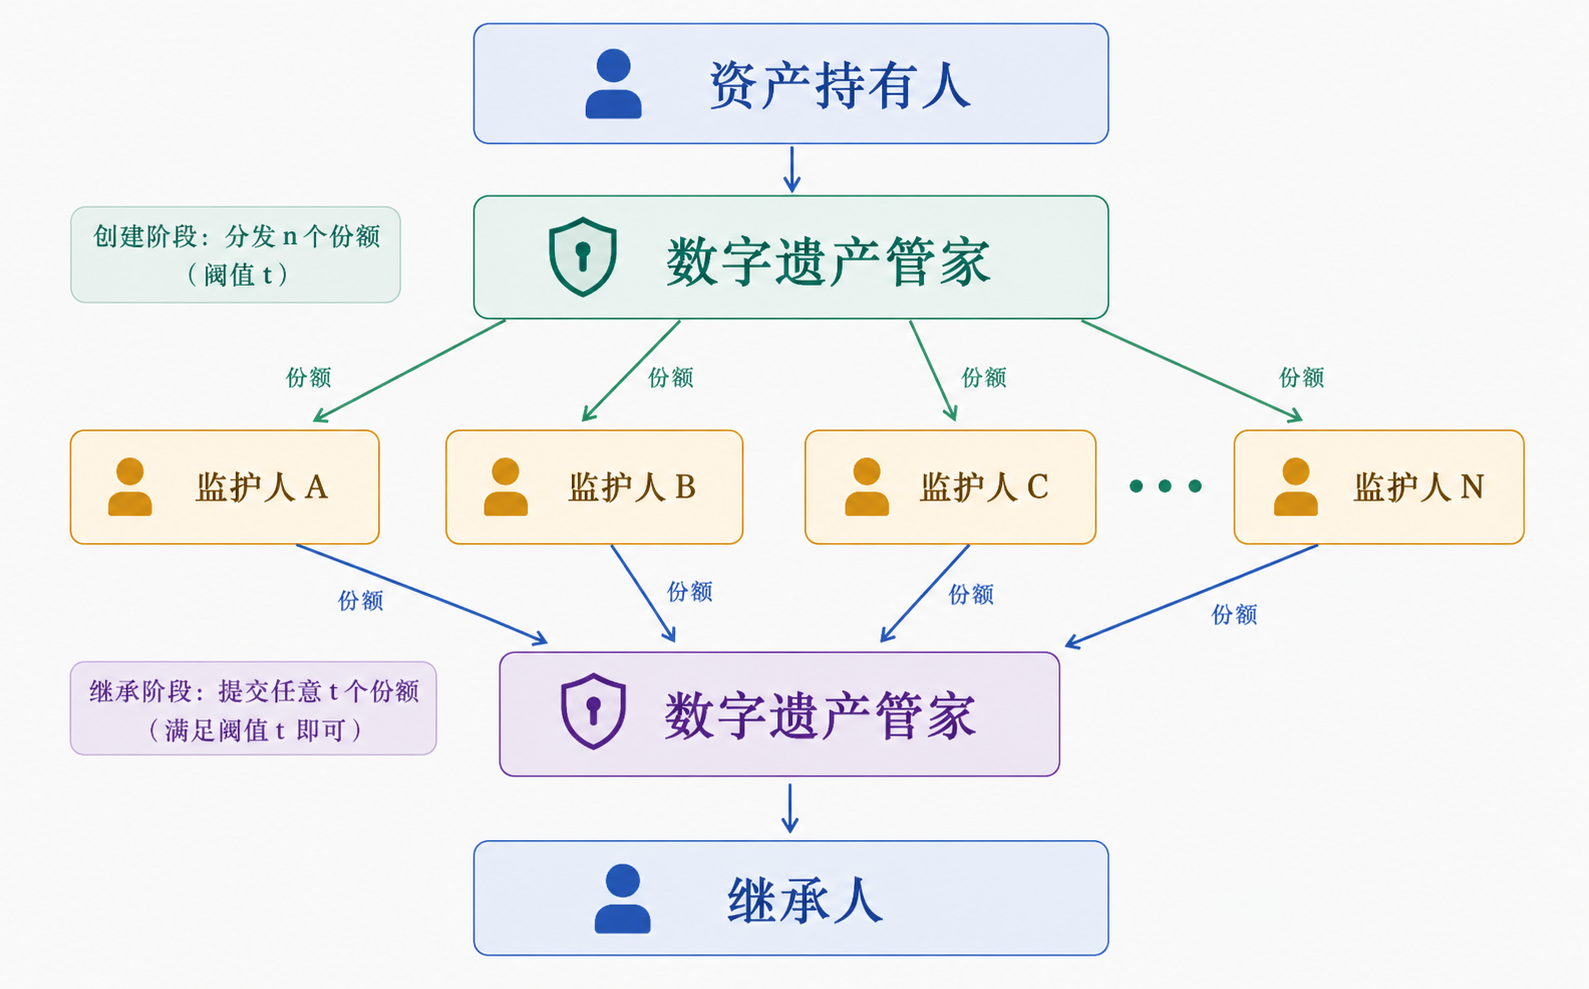
\includegraphics[width=1.0\textwidth]{figures/fig_overview.png}
	\caption{\project 系统全景：密钥拆分为$n$份额分发给监护人，资产加密后交后端存储；继承时达到$t$份额即可恢复}
	\label{fig:overview}
\end{figure}

% ==================== 第二章 作品设计与实现 ====================
\chapter{作品设计与实现}

\section{总体架构}

系统按照用户层、API层、核心服务层、存储层、智能合约层进行分层设计。各层职责明确，层间通过明确的接口进行通信。以下沿数据流方向——从用户操作到资产落盘——逐层描述各层职责及层间安全边界。

\begin{figure}[H]
\centering
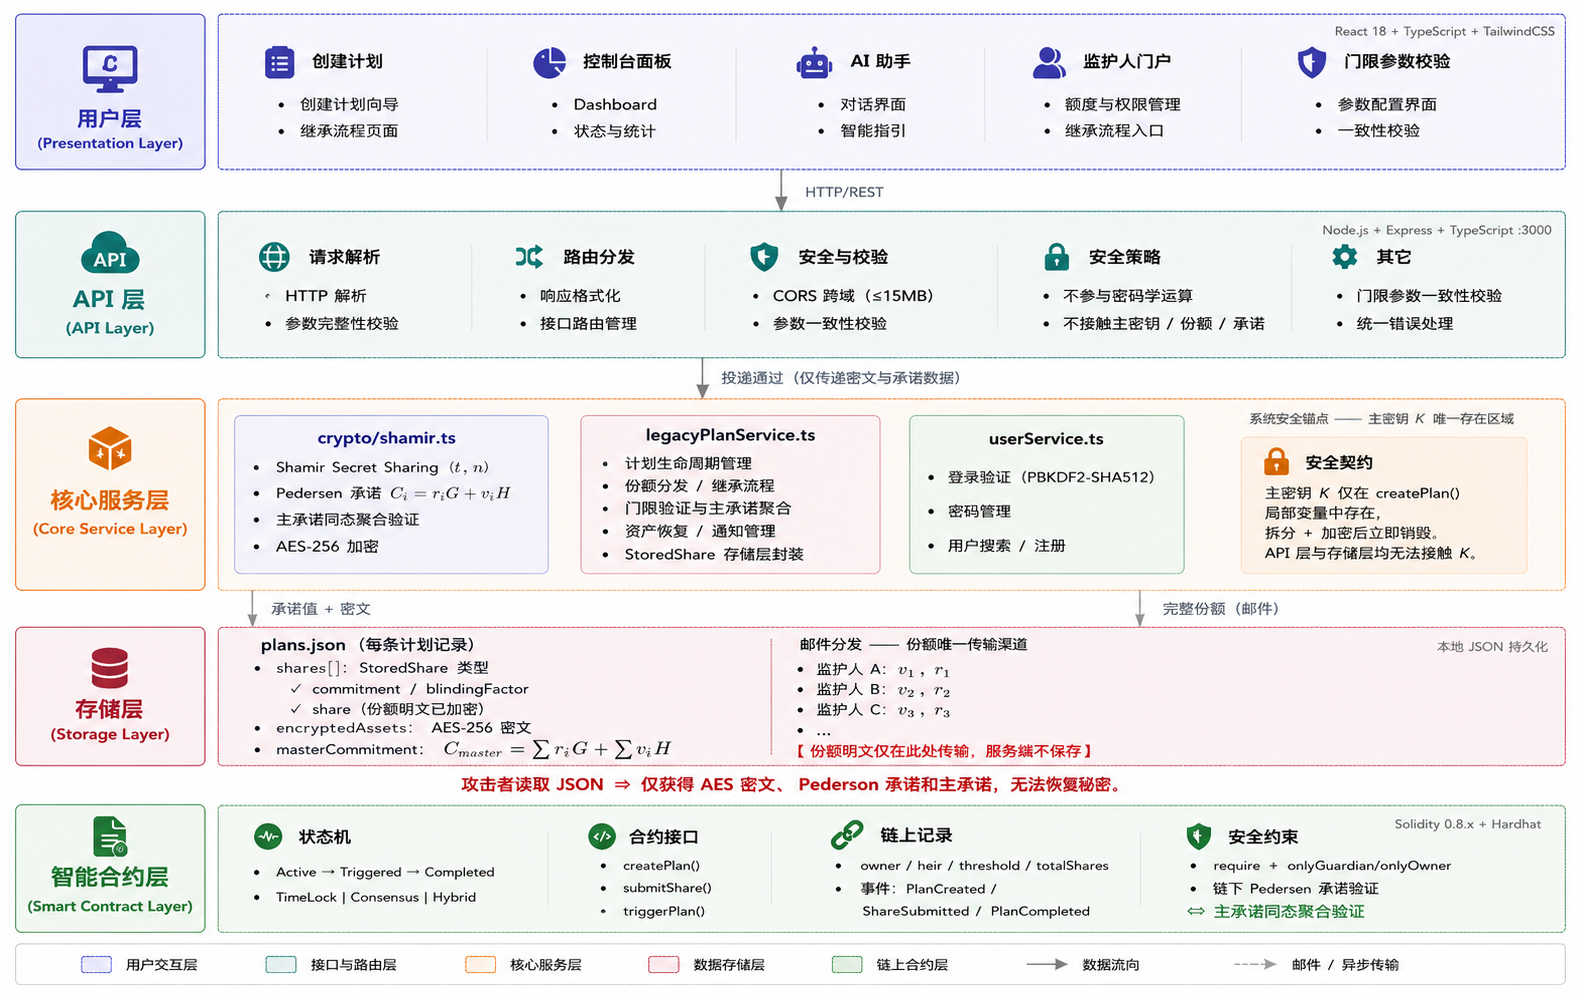
\includegraphics[width=1.0\textwidth]{figures/picture2.1.png}
\caption{系统总体架构示意：用户层、API层、核心服务层、存储层与智能合约层的分层关系及层间数据流向}
\label{fig:overview_arch}
\end{figure}

\textbf{用户层（Presentation Layer）。}基于React 18 + TypeScript + TailwindCSS构建的单页面应用，使用Vite构建。该层提供创建计划四步向导、控制台面板、继承流程页面、监护人门户和AI助手对话框等可视化界面。用户在向导中配置资产、监护人和门限参数后，前端对门限参数实施第一轮校验（threshold $\ge$ 1、threshold $\le$ totalShares、totalShares $\le$ guardians.length），随后将请求发送至API层。采用Framer Motion实现页面过渡动画，降低门限密码学配置的专业感知门槛。

\textbf{API层（API Layer）。}基于Node.js + Express + TypeScript构建的RESTful API服务，监听3000端口。该层负责HTTP请求解析、参数完整性校验、路由分发和响应格式化。使用CORS中间件支持跨域请求，JSON body大小限制为15MB以支持文件上传场景。API层对门限参数实施与前端一致的第二轮校验（与前端形成双重验证闭环），校验通过后将请求转发至核心服务层；API层自身不参与任何密码学运算，不接触主密钥、份额值或承诺材料。

\textbf{核心服务层（Core Service Layer）。}系统安全的核心锚点位于此层，包含三个子模块。密码学模块（crypto/shamir.ts）负责Shamir秘密共享（在secp256k1标量域$\mathbb{F}_q$上构造双多项式）、Pedersen同态承诺（$C_i = r_iG + v_iH$）、零和多项式份额刷新、AES-256资产加解密以及ECIES份额传输加密。业务服务模块（services/legacyPlanService.ts）负责遗产计划的生命周期编排——接收API层转发的请求，调用密码学模块执行拆分与承诺生成，将不含份额明文的StoredShare（仅保留承诺值、盲因子、胁迫承诺）写入存储层，并通过邮件服务将完整份额值发送给监护人。用户服务模块（services/userService.ts）负责PBKDF2-SHA512密码哈希、登录验证码生成和用户搜索。该层的核心安全契约是：主密钥$K$仅在createPlan方法的局部变量中存在，完成拆分和资产加密后立即超出作用域——API层和存储层自始至终无法接触$K$。

\textbf{存储层（Storage Layer）。}使用本地JSON文件进行持久化，管理plans.json、requests.json、users.json和verificationCodes.json四个数据文件。每条遗产计划记录包含加密资产包（encryptedAssets，AES密文）、份额承诺数组（shares，StoredShare类型，仅含commitment、blindingFactor、duressCommitment，不含value）和主承诺（masterCommitment，$C_{\text{master}} = RG + sH$）。该层的安全边界是：攻击者即使获得四个JSON文件的完整副本，也只能看到密文和公开承诺值——解密需要主密钥$K$，恢复$K$需要至少$t$个监护人的份额明文值，而份额明文仅存在于监护人的邮件中，从未进入存储层。

\textbf{智能合约层（Smart Contract Layer）。}基于Solidity 0.8.x编写的LegacyContract合约，定义PlanStatus（Active $\to$ Triggered $\to$ Completed）状态机和TriggerMode（TimeLock、Consensus、Hybrid）触发模式。合约在链上记录计划元信息（owner、heir、threshold、totalShares）、监护人地址与承诺值（bytes32）的映射、份额提交状态以及状态转换事件（PlanCreated、ShareSubmitted、PlanTriggered、PlanCompleted，均以indexed修饰）。合约层的状态约束（require前置条件 + onlyGuardian/onlyOwner修饰符）可作为独立的链上校验模块。当前合约已在 Hardhat 本地网络通过功能测试，后端的继承流程通过本地 JSON 文件管理计划状态；合约与后端 API 的集成已预留接口，可作为后续去中心化部署的基础。


\begin{figure}[H]
\centering
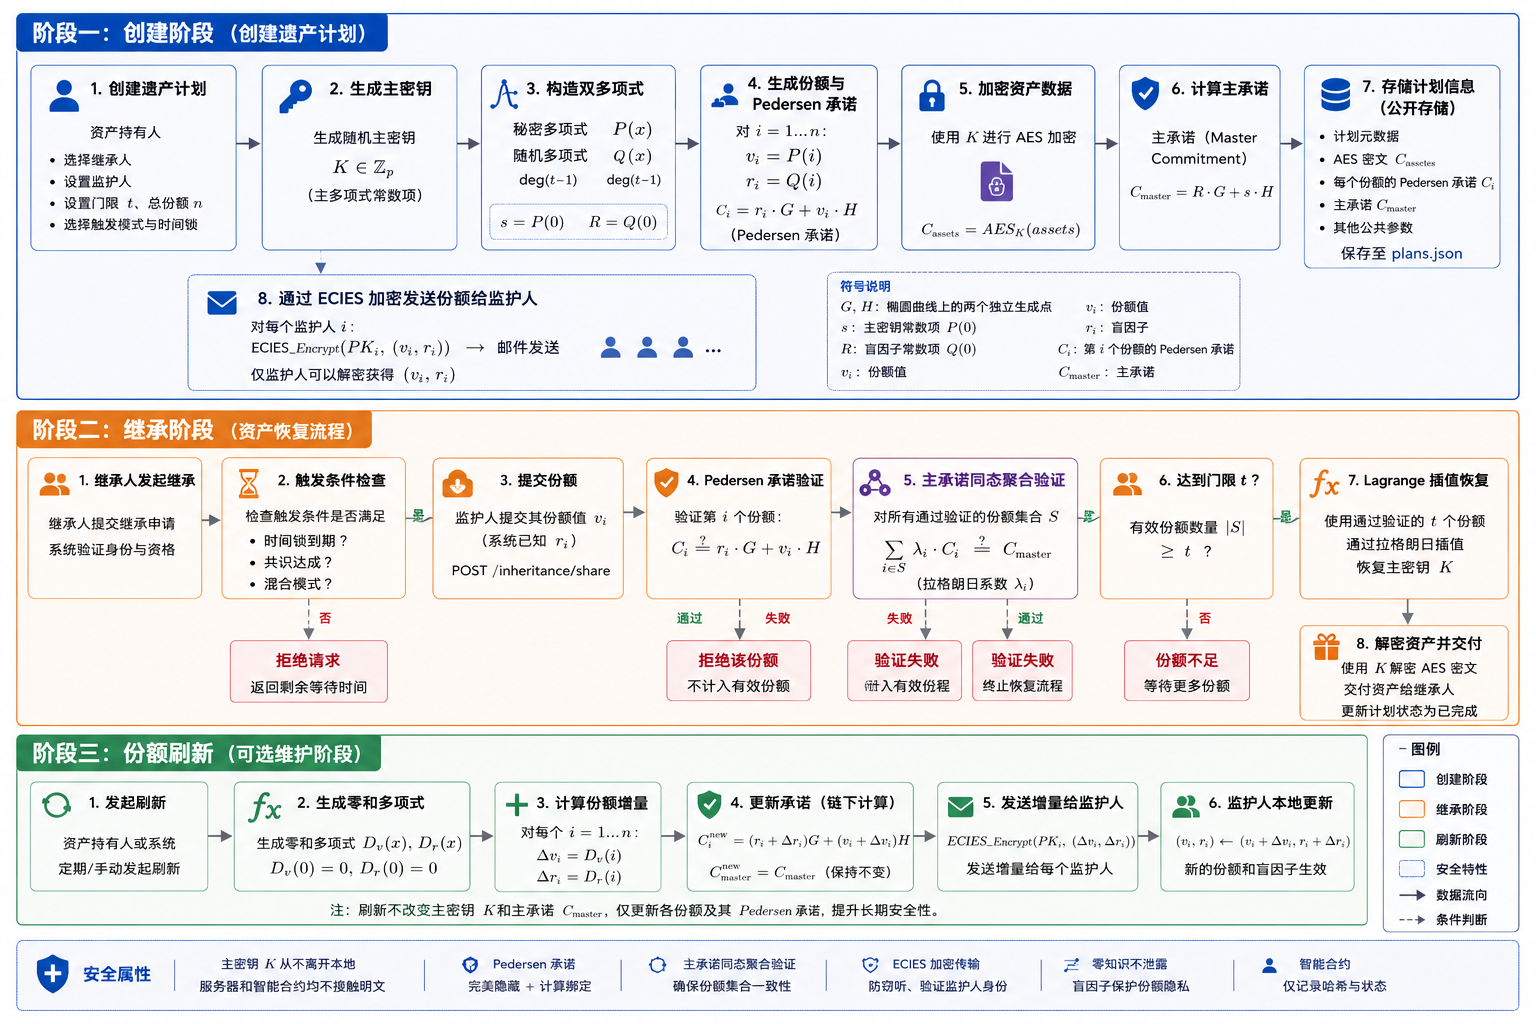
\includegraphics[width=1.0\textwidth]{figures/flowchart.png}
\caption{系统完整协议流程——创建阶段、继承阶段与同态份额刷新阶段}
\label{fig:flowchart}
\end{figure}

\subsection{后端LegacyPlan结构}

后端LegacyPlan结构是整个系统的核心数据模型。其最关键的安全设计是shares字段使用StoredShare类型而非完整的Share类型——StoredShare仅保存份额标识、索引、椭圆曲线承诺值和盲因子，不保存份额明文值value。这意味着即使攻击者获得服务器数据库的完全读取权限，也无法直接获得用于恢复主密钥的份额值。

\begin{lstlisting}[caption={后端计划核心结构定义 (legacyPlanService.ts:45-61)}]
export interface LegacyPlan {
  id: string
  name: string
  assets: any[]                   // 资产摘要信息
  guardians: any[]                // 监护人信息（含邮箱）
  threshold: number               // 恢复门限t
  totalShares: number             // 总份额数n
  triggerMode: 'consensus' | 'timed'  // 触发模式
  timeLock: number                // 时间锁天数
  shares: StoredShare[]           // 不含value的安全份额结构
  encryptedAssets: string         // AES加密的资产包
  masterCommitment: string        // C_master = R*G + s*H（同态验证）
  createdAt: string
  updatedAt: string
  status: 'active' | 'collecting' | 'completed'
  creatorId?: string
\end{lstlisting}

\subsection{Share与StoredShare的差分设计}

系统在密码学模块中定义了两种份额接口：Share包含完整的份额信息（value字段）用于临时计算和监护人交付；StoredShare剔除value字段仅保留承诺值和盲因子（blindingFactor），用于持久化存储。盲因子保留是为了在监护人提交份额时能够重算 Pedersen 承诺进行单点验证；份额明文 value 则仅在创建时通过邮件发送给监护人，不进入存储层。这一差分设计是系统”最小化存储敏感数据”核心安全原则的体现——即使攻击者获得plans.json的完全读取权限，也无法获取份额明文值。

StoredShare接口定义如下（shamir.ts:13-20）：

\begin{lstlisting}[caption={StoredShare安全份额结构 (shamir.ts:13-20)}]
export interface StoredShare {
  id: string
  index: number
  commitment: string           // Pedersen承诺 C_i = r_i*G + v_i*H
  blindingFactor: string       // 盲因子 r_i（提交时重算承诺用）
  duressCommitment?: string    // 胁迫承诺
  duressBlindingFactor?: string // 胁迫盲因子
}
\end{lstlisting}

\subsection{InheritanceRequest结构}

继承请求结构跟踪继承流程的状态演进，包含initiatorId、heirEmail、sharesCollected、submittedGuardians（防重数组）等字段。关键安全设计：submittedShares字段仅在内存中暂存不持久化到JSON文件，达到门限后立即用于恢复主密钥并解密资产。

\section{创建遗产计划完整流程}

创建遗产计划是系统的核心业务流程入口。本节从前端交互、后端参数校验、密码学拆分、承诺生成、加密存储和份额分发六个阶段详细描述该流程。

\subsection{前端多步骤向导}

前端CreatePlan页面采用四步向导设计，逐步引导用户完成资产配置、监护人设置、触发条件配置和确认创建。每步包含实时表单验证和错误提示，降低用户配置门限密码学参数的专业门槛。

第一步“添加资产”支持四种资产类型（加密货币、云账号、加密文件、智能合约），每种类型有对应的输入格式校验规则。文件类型资产支持通过FileReader API进行本地Base64编码后上传。第二步“设置监护人”集成了用户搜索功能，通过调用/api/users/search接口查找已注册用户，自动填充监护人ID、姓名和邮箱。同时允许指定继承人。第三步“设置触发条件”可选社会共识模式或时间锁模式（混合模式），实时展示门限配置为t-of-n含义的解释文本。第四步“确认创建”展示资产清单和监护人配置摘要，并提供安全提示。

\subsection{后端创建流程}

当后端API收到创建计划请求后，按以下步骤处理：

\begin{enumerate}
  \item \textbf{参数校验：}验证资产列表非空、监护人列表非空、门限$t$满足$1 \le t \le n$、总份额数不超过监护人数量。
  \item \textbf{主密钥生成：}调用shamirSecretSharing.generateMasterKey()生成256位随机主密钥$K$。该方法使用拒绝采样在secp256k1标量域$\mathbb{F}_q$内生成均匀分布的随机数。
  \item \textbf{秘密共享拆分：}以主密钥$K$为$a_0$，生成$t-1$个随机系数$a_1,\dots,a_{t-1}$，构造$t-1$次多项式$f(x)=a_0+a_1x+\cdots+a_{t-1}x^{t-1} \pmod{q}$。对$i=1$到$n$，计算$y_i=f(i)$，得到$n$个份额点$(i, y_i)$。
  \item \textbf{承诺生成：}利用双多项式结构为每个份额计算 Pedersen 承诺$C_i = r_iG + v_iH$，其中$v_i = P(i)$来自份额值多项式，$r_i = Q(i)$来自盲因子多项式。同时生成主承诺$C_{\text{master}} = RG + sH$（$s$为主密钥，$R$为主盲因子）用于后续同态聚合验证，并为每个份额生成独立的胁迫码信息用于抗胁迫检测。承诺用于后续验证份额完整性。
  \item \textbf{资产加密：}调用CryptoJS.AES.encrypt()以主密钥$K$加密整个资产包JSON字符串，得到密文$C$。
  \item \textbf{安全存储：}将Share对象转换为StoredShare（移除value字段），与资产摘要、监护人信息、加密资产包等组装为LegacyPlan结构，持久化到plans.json。
  \item \textbf{份额分发：}通过邮件服务将包含value的完整份额信息发送给各监护人。邮件中包含计划名称、计划ID、份额ID、份额索引、份额值、门限和总份额数等关键信息。
\end{enumerate}

\subsection{创建计划关键代码}

createPlan方法按六步流水线执行：输入验证 $\to$ generateMasterKey生成256位主密钥 $\to$ shamirSecretSharing.split进行门限拆分 $\to$ encryptAsset以主密钥加密资产包 $\to$ Share转StoredShare（关键安全步骤：移除value字段后持久化）$\to$ sendShareEmails通过邮件向监护人分发完整份额。该方法体现了"主密钥仅在内存中存在、拆分后立即丢弃、持久化存储不含份额明文"的安全设计原则。

\section{Shamir秘密共享实现}

Shamir Secret Sharing是本作品的密码学基础。\textbf{技术选型论证：}在门限秘密共享方案中，Blakley方案基于超平面几何构造但份额尺寸随门限线性增长，基于XOR的简单拆分不具备门限灵活性。选择Shamir方案的理由有三：（1）\textbf{信息论安全}——任意$t-1$个份额不给攻击者提供关于秘密的任何信息，这一保证不依赖任何计算复杂性假设，适用于跨越数十年的数字遗产继承场景；（2）\textbf{参数灵活性}——$n$和$t$可独立设置，支持2-of-3到10-of-15等任意配置；（3）\textbf{代数结构兼容}——Shamir多项式在有限域上的运算可直接与Pedersen承诺的椭圆曲线同态性质结合，支撑可验证秘密共享和同态份额刷新。

\subsection{数学原理}

Shamir秘密共享的核心思想是在有限域$\mathbb{F}_q$上构造$t-1$次随机多项式：
\[
f(x)=a_0+a_1x+a_2x^2+\cdots+a_{t-1}x^{t-1}\pmod{q}
\]
其中秘密$S=a_0=f(0)$。系统随机生成$t-1$个系数$a_1,\dots,a_{t-1}$，为$n$个参与者分别计算份额点$(x_i, y_i=f(x_i))$。由于$t-1$次多项式由$t$个点唯一确定，任意$t$个份额可以重构多项式并计算$f(0)$恢复秘密；而任意$t-1$个份额只提供$t-1$个点，无法唯一确定$t-1$次多项式，因此从信息论角度获得的信息量为零。

恢复阶段使用拉格朗日插值公式：
\[
S = f(0) = \sum_{i=1}^{t} y_i \prod_{j \neq i} \frac{0-x_j}{x_i-x_j} = \sum_{i=1}^{t} y_i \prod_{j \neq i} \frac{-x_j}{x_i-x_j} \pmod{q}
\]

本作品在使用域方面有一个关键设计决策：没有混用椭圆曲线基域和群阶，而是在secp256k1的标量域$\mathbb{F}_q$（其中$q$为群阶）上进行Shamir多项式运算。这使得Pedersen承诺中的椭圆曲线等式自然成立，无需额外的域兼容性处理。

\subsection{代码实现}

\begin{lstlisting}[caption={双多项式Shamir秘密共享实现 (shamir.ts:92-115), label={lst:split}}]
split(secret: string, n: number, t: number): Share[] {
  const secretNum = BigInt('0x' + secret)
  const coefficients: bigint[] = [secretNum]

  for (let i = 1; i < t; i++) {
    coefficients.push(this.generateRandomCoefficient())
  }

  const shares: Share[] = []
  for (let i = 1; i <= n; i++) {
    const x = BigInt(i)
    const y = this.evaluatePolynomial(coefficients, x)
    const share: Share = {
      id: uuidv4(),
      index: i,
      value: y.toString(16),
      commitment: '',
    }
    share.commitment = this.generateCommitment(share)
    shares.push(share)
  }

  return shares
}
\end{lstlisting}

系统在实际创建计划时调用\texttt{generatePedersenShares}（shamir.ts:231-258）而非上述基础\texttt{split}方法。该方法在两个独立的Shamir多项式——份额值多项式$P(x)$（常数项为主密钥$s$）和盲因子多项式$Q(x)$（常数项为随机主盲因子$R$）——上同时求值，得到每份份额的$(v_i, r_i)$对，为后续Pedersen承诺生成和同态聚合验证提供密码学基础。

多项式求值采用逐项累加在$O(t)$次模乘内完成；份额合并采用拉格朗日插值在有限域上的直接实现，使用扩展欧几里得算法计算模逆元。图\ref{fig:shamir_poly}以$t=3,n=4$为例展示了多项式构造与恢复的几何直观。

\begin{figure}[H]
\centering
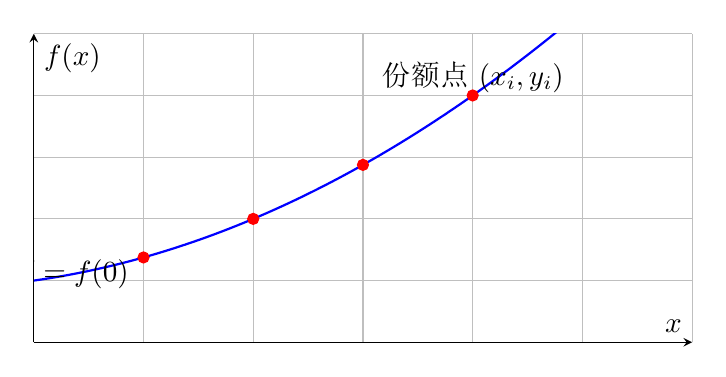
\includegraphics[width=1.0\textwidth]{figures/fig_shamir_poly.png}
\caption{Shamir秘密共享多项式示意图（t=3, n=4）：任意3个点可唯一确定二次多项式并恢复S=f(0)}
\label{fig:shamir_poly}
\end{figure}

\subsection{随机标量生成}

密码学安全随机数生成是整个系统安全性的基石之一。本作品使用Node.js的crypto.randomBytes（底层调用操作系统密码学安全随机源）配合拒绝采样在有限域$\mathbb{F}_q$内生成均匀分布的随机标量，避免简单取模带来的微小偏差。在secp256k1的256位标量域中，拒绝概率约为$2^{-128}$量级，期望采样次数接近1。

\section{Pedersen同态承诺与双多项式结构}

\subsection{Pedersen同态承诺}

前述Shamir秘密共享实现了密钥的门限拆分与恢复，但server需要验证监护人提交的份额是否正确，又不能直接看到份额值（否则server即可自行恢复主密钥）。Pedersen承诺解决了这一矛盾——在公开份额承诺的同时隐藏份额值本身。

\noindent \textbf{技术选型论证：}在可验证秘密共享的承诺方案中，Feldman的VSS使用$y_iG$作为承诺——计算简单但仅有计算隐藏性（攻击者若在未来破解离散对数，可从承诺反推份额值）。Benaloh的承诺具有同态性但需在合数阶群上工作，参数生成复杂。选择Pedersen承诺的理由有三：（1）\textbf{完美隐藏}——承诺$C$在信息论层面不泄露$v$的任何比特信息，不依赖离散对数假设，适合长期数字遗产场景；（2）\textbf{同态加法}——$C(v_1,r_1)+C(v_2,r_2)=C(v_1+v_2,r_1+r_2)$是实现同态份额刷新和主承诺验证的代数基础；（3）\textbf{椭圆曲线实现}——构建于secp256k1之上，与比特币/以太坊共享相同密码学基础设施，便于未来的链上验证。

\noindent \textbf{承诺公式}。给定secp256k1椭圆曲线上两个独立的生成点$G$和$H$（$H = G \cdot \text{SHA256}(\text{seed})$，离散对数关系未知），对份额值$v$和盲因子$r$的承诺为：

\[
C(v, r) = r \cdot G + v \cdot H
\]

\noindent \textbf{安全属性}：
\begin{itemize}
  \item \textbf{完美隐藏}（Perfect Hiding）：对于任意$C$和任意$v$，存在$r$使得$C = rG + vH$，即$C$不泄露$v$的任何信息。
  \item \textbf{计算绑定}（Computational Binding）：找到不同的$(r', v')$使得$C(r', v') = C(r, v)$等价于解椭圆曲线上的离散对数问题$\log_G H$。
\end{itemize}

\noindent \textbf{同态加法性质}：
\[
C(v_1, r_1) + C(v_2, r_2) = C(v_1 + v_2, r_1 + r_2)
\]

这一性质是份额刷新功能的核心密码学基础。

\subsection{双多项式份额结构}

标准Shamir方案仅拆分份额值，无法在不暴露值的情况下验证份额正确性。本系统引入\textbf{第二个盲因子多项式}$Q(x)$，构成双多项式结构：

\[
\begin{cases}
P(x) = s + a_1x + a_2x^2 + \cdots + a_{t-1}x^{t-1} \pmod{q} \\
Q(x) = R + b_1x + b_2x^2 + \cdots + b_{t-1}x^{t-1} \pmod{q}
\end{cases}
\]

其中$P(0) = s$（主密钥），$Q(0) = R$（随机主盲因子）。份额$i$包含值$v_i = P(i)$和盲因子$r_i = Q(i)$。对应的Pedersen承诺为$C_i = r_iG + v_iH$。\textbf{主承诺}$C_{\text{master}} = RG + sH$公开存储。

\noindent \textbf{同态可验证性}——利用Lagrange系数$\lambda_j$在EC点上直接运算：

\[
\Sigma(\lambda_j \cdot C_{i_j}) = C_{\text{master}}
\]

任意第三方（包括server）可验证一组份额是否正确对应主密钥，无需知道份额值$v_i$和盲因子$r_i$。

\subsection{同态份额刷新（零和多项式）}

\textbf{创新点}：在server\textbf{完全不存储主密钥}的前提下，实现安全的份额刷新轮换。由于主密钥在创建后立即销毁，传统的"解密$\to$重新拆分"方法不可用。

\noindent \textbf{原理}。生成两个$t-1$次零和多项式$Z_v(x)$和$Z_r(x)$，满足$Z_v(0) = Z_r(0) = 0$：

\begin{itemize}
  \item 新份额值$v'_i = v_i + Z_v(i)$（监护人本地计算）
  \item 新盲因子$r'_i = r_i + Z_r(i)$（监护人本地计算）
  \item 新承诺$C'_i = C_i + Z_r(i)\cdot G + Z_v(i)\cdot H$（server公开计算，纯EC点运算）
  \item 主承诺不变$C'_{\text{master}} = C_{\text{master}}$（因为$Z(0) = 0$）
\end{itemize}

零和多项式每次刷新随机生成，一次有效。与需存储主密钥的传统方案相比，本方法具有以下安全优势：

\begin{table}[H]
\centering
\caption{同态刷新与传统方案的安全对比}
\begin{tabularx}{\textwidth}{lXc}
\toprule
对比项 & 传统方案（需存储主密钥） & 本方案（同态刷新）\\
\midrule
Server密钥存储 & 需加密存储主密钥 & 全程不接触主密钥\\
刷新计算 & 解密$\to$重拆分$\to$重新加密 & 纯EC点运算\\
通信内容 & 发送完整新份额（机密） & 仅发送公开增量\\
安全性 & 密钥泄露$\to$全盘暴露 & 零和多项式一次有效\\
\bottomrule
\end{tabularx}
\end{table}

\noindent 核心代码实现如下：

\begin{lstlisting}[caption={零和多项式同态刷新增量生成 (shamir.ts)}]
generateRefreshDeltas(n: number, t: number): ShareDelta[] {
  const zvCoeffs: bigint[] = [BigInt(0)]    // Z_v(0) = 0
  const zrCoeffs: bigint[] = [BigInt(0)]    // Z_r(0) = 0
  for (let i = 1; i < t; i++) {
    zvCoeffs.push(generateRandomCoefficient())
    zrCoeffs.push(generateRandomCoefficient())
  for (let i = 1; i <= n; i++) {
    const x = BigInt(i)
    deltas.push({
      index: i,
      valueDelta: evaluatePoly(zvCoeffs, x).toString(16),
      blindingDelta: evaluatePoly(zrCoeffs, x).toString(16),
    })
  return deltas
\end{lstlisting}

\begin{lstlisting}[caption={承诺同态刷新计算 (shamir.ts)}]
computeRefreshedCommitment(oldCommitment: string,
    valueDelta: string, blindingDelta: string): string {
  const G = this.ec.g, H = this.getH()
  const oldPoint = this.ec.keyFromPublic(oldCommitment, 'hex').getPublic()
  const vDeltaBN = new BN(valueDelta, 16)
  const rDeltaBN = new BN(blindingDelta, 16)
  // C' = C + delta_r*G + delta_v*H
  const newPoint = oldPoint.add(G.mul(rDeltaBN)).add(H.mul(vDeltaBN))
  return newPoint.encode('hex', false)
\end{lstlisting}

\section{主承诺同态聚合验证}

单点验证（见 §2.4）确保每个份额值本身未被篡改，但仍存在一个理论上的边缘情况：攻击者可能从多个不同计划中分别获取合法份额（每个份额各自通过单点验证），凑齐 $t$ 个份额后提交。这些份额虽然在各自计划中是合法的，但来源于不同的秘密共享实例，插值结果将不是任何一个计划的主密钥。

主承诺同态聚合验证利用Lagrange插值与Pedersen承诺的同态性质，在不需要知晓份额值的前提下，验证一组份额是否确实对应创建时生成的主密钥。

\subsection{验证原理}

创建计划时，系统利用 §2.4.2 所述的双多项式结构生成主承诺：
\[
C_{\text{master}} = R \cdot G + s \cdot H
\]
其中 $s = P(0) = \text{masterKey}$，$R = Q(0)$ 为主盲因子。$C_{\text{master}}$ 公开存储在 LegacyPlan.masterCommitment 字段中。

恢复阶段收集到 $t$ 个份额后，利用 Lagrange 插值公式在椭圆曲线上做同态运算。由于 $P(x)$ 和 $Q(x)$ 共享同一组 Lagrange 系数 $\lambda_i$，有：
\[
s = P(0) = \sum_{i=1}^{t} \lambda_i \cdot P(i) = \sum_{i=1}^{t} \lambda_i \cdot v_i
\]
\[
R = Q(0) = \sum_{i=1}^{t} \lambda_i \cdot Q(i) = \sum_{i=1}^{t} \lambda_i \cdot r_i
\]

利用 Pedersen 承诺的同态加法性质（§2.4.1），在椭圆曲线上直接验证：
\[
\sum_{i=1}^{t} \lambda_i \cdot C_i =
\left(\sum_{i=1}^{t} \lambda_i r_i\right) G +
\left(\sum_{i=1}^{t} \lambda_i v_i\right) H =
R \cdot G + s \cdot H = C_{\text{master}}
\]

验证方程成立当且仅当这 $t$ 个份额确实来源于同一个秘密共享实例。整个计算过程仅涉及椭圆曲线点加法和标量乘法，无需知晓任何份额值或盲因子。

\subsection{代码实现}

\begin{lstlisting}[caption={主承诺同态聚合验证 (shamir.ts:271-314, 节选)}]
verifyMasterCommitment(
  shares: Array<{ index: number; commitment: string }>,
  masterCommitment: string
): boolean {
  const t = shares.length
  if (t < 1) return false

  const sorted = [...shares].sort((a, b) => a.index - b.index)
  const curveN = this.ec.curve.n
  const G = this.ec.g

  // 从无穷远点开始累加
  let sum = G.mul(new BN(0))

  for (let i = 0; i < t; i++) {
    const idx = sorted[i].index
    const point = this.ec.keyFromPublic(
      sorted[i].commitment, 'hex').getPublic()

    // 计算 Lagrange 系数 lambda_i
    let lambda = new BN(1)
    for (let j = 0; j < t; j++) {
      if (i !== j) {
        const num = new BN(0).sub(
          new BN(sorted[j].index)).umod(curveN)
        const den = new BN(idx).sub(
          new BN(sorted[j].index)).umod(curveN)
        lambda = lambda.mul(num).mul(
          den.invm(curveN)).mod(curveN)
      }
    }
    // sum += lambda_i * C_i
    sum = sum.add(point.mul(lambda))
  }

  if (sum.isInfinity()) return false
  return sum.encode('hex', false) === masterCommitment
}
\end{lstlisting}

\subsection{与单点验证的互补关系}

\begin{table}[H]
\centering
\caption{两层验证机制对比}
\begin{tabularx}{\textwidth}{p{2.8cm}XX}
\toprule
 & Pedersen 单点验证（§2.4） & 主承诺同态聚合验证 \\
\midrule
验证对象 & 单个份额 & $t$ 个份额的集合 \\
验证内容 & 份额值是否与承诺匹配 & 份额集合是否对应主密钥 \\
所需数据 & $r_i$（盲因子） & $C_{\text{master}}$（主承诺） \\
数学基础 & 离散对数困难 & Lagrange 插值 + 同态加法 \\
阻止的攻击 & 值篡改、随机伪造 & 跨实例份额注入 \\
触发时机 & 监护人每次提交时 & 达到门限后可调用 \\
\bottomrule
\end{tabularx}
\end{table}

两层验证形成互补：第一层在每个监护人提交时即时拦截伪造数据；第二层在收集到 $t$ 个份额后确认集合来源一致——利用 Lagrange 系数的加权和绑定到 $C_{\text{master}}$，任何来自不同多项式的份额即使单独通过单点验证，其聚合结果也无法匹配创建时生成的主承诺。两层验证任一失败均阻止密钥恢复和资产解密。

\begin{figure}[H]
\centering
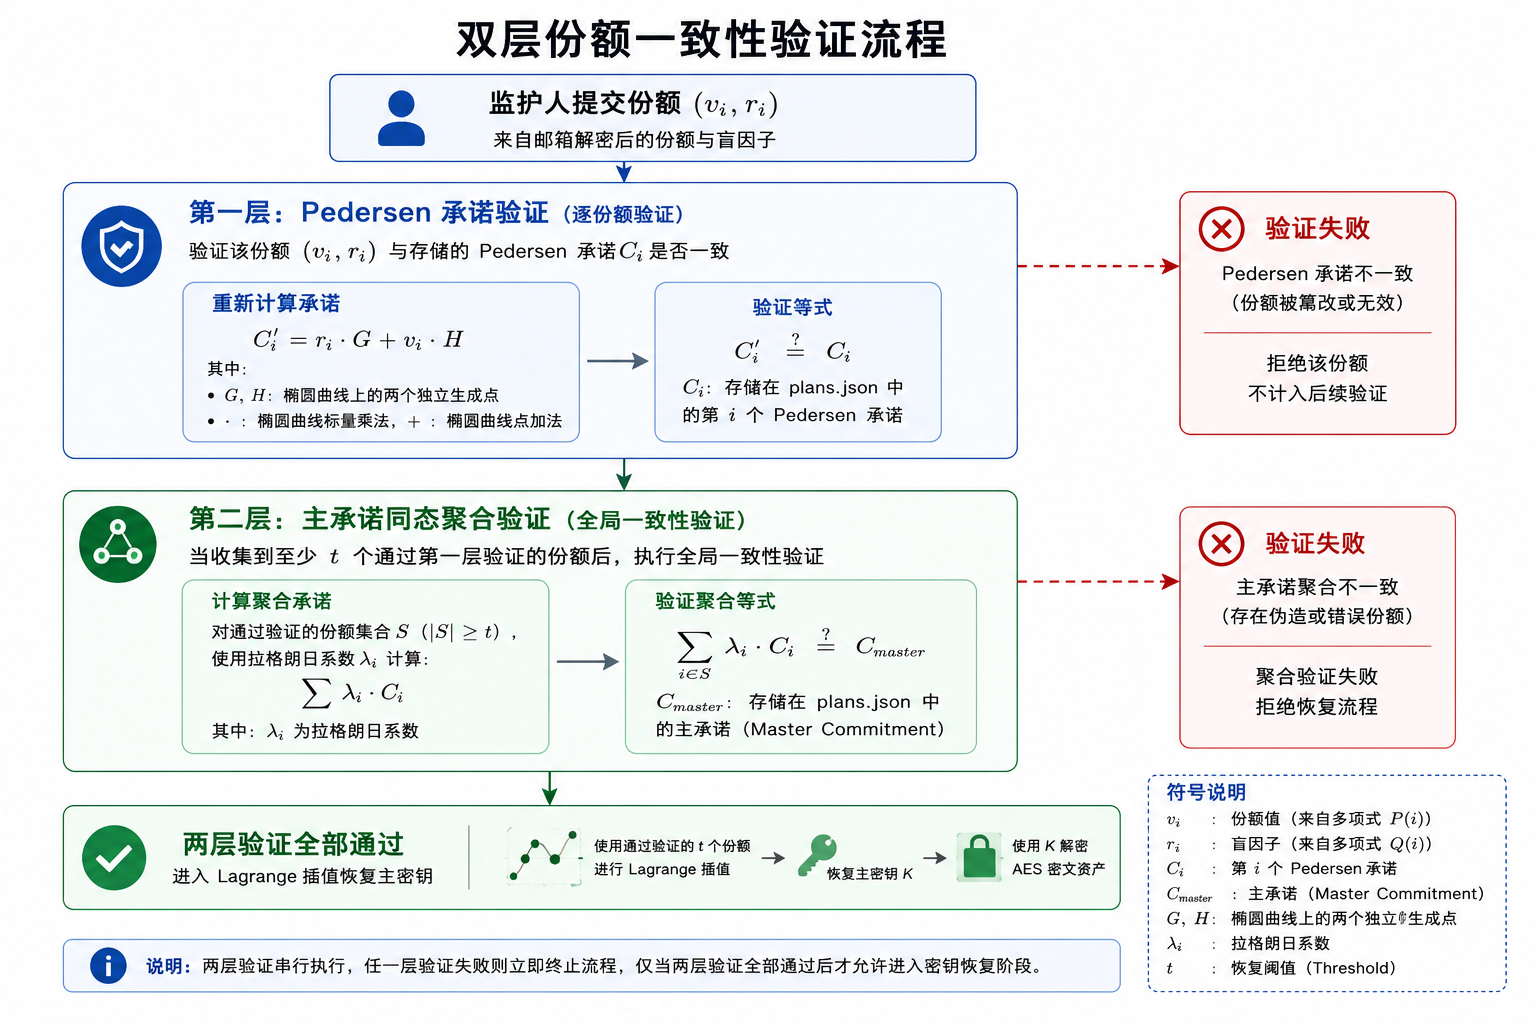
\includegraphics[width=1.0\textwidth]{figures/fig_verifypipe.png}
\caption{两层份额验证机制：单点验证在提交时即时拦截伪造，同态聚合验证在收集完毕后确认来源一致}
\label{fig:verifypipe}
\end{figure}


\section{资产加密与恢复}

为避免数字资产直接暴露在数据库或服务器中，本作品采用“对称加密+门限恢复”的双层安全架构。资产信息（可能包含私钥、助记词、账号密码等高度敏感数据）在进入存储前即被加密，而加密密钥本身又通过秘密共享拆分为多个份额。

\subsection{加密层设计}

系统生成随机主密钥$K$后，利用AES对称加密算法对整个资产集合进行加密：

\begin{lstlisting}[caption={AES加密与解密 (shamir.ts:135-143)}]
encryptAsset(assets: any[], masterKey: string): string {
  const assetsString = JSON.stringify(assets)    // 序列化为JSON
  return CryptoJS.AES.encrypt(assetsString, masterKey).toString()

decryptAsset(encryptedAsset: string, masterKey: string): any[] {
  const bytes = CryptoJS.AES.decrypt(encryptedAsset, masterKey)
  const decryptedString = bytes.toString(CryptoJS.enc.Utf8)
  return JSON.parse(decryptedString)
\end{lstlisting}

加密后得到的密文$C=\text{AES}_K(M)$被持久化存储在LegacyPlan.encryptedAssets字段中。此时数据库仅保存$C$而不保存$K$——$K$在创建计划时仅短暂存在于内存中，随后作为Shamir秘密共享的秘密输入被拆分，自身即被丢弃。

\subsection{门限层设计}

主密钥$K$作为Shamir秘密共享的秘密$S=K$被拆分为$n$个份额。份额分发后，$K$的单份完整副本不再存在于任何地方——必须收集至少$t$个有效份额才能通过拉格朗日插值恢复$K$。

从信息论角度，当收集的份额数$m<t$时：
\[
I(K; \text{Share}_{i_1}, \dots, \text{Share}_{i_m}) = 0
\]
即不足门限的参与者获得的信息量与秘密$K$之间的互信息为零——他们无法推断任何关于$K$的信息。

\subsection{恢复链路}

继承触发后的完整资产恢复链路为：
\[
\begin{aligned}
&\text{继承触发}\rightarrow\text{监护人提交份额}\rightarrow\text{验证机制}\\
&\qquad\rightarrow\text{收集至}t\text{个份额}\rightarrow\text{拉格朗日插值恢复}K\\
&\qquad\rightarrow\text{AES解密}C\text{得}M\rightarrow\text{交付继承人}
\end{aligned}
\]

在实现层面，当submitGuardianShare检测到sharesCollected达到阈值后，立即执行恢复和解密：

\begin{lstlisting}[caption={达到门限后的自动恢复 (legacyPlanService.ts:575-601, 节选)}]
if (request.sharesCollected >= plan.threshold) {
  if (request.hasDuress) {
    // 检测到胁迫提交：不恢复资产，通知监护人
    request.status = 'duress'
    this.sendDuressAlerts(plan)
  } else {
    request.status = 'verifying'
    plan.status = 'completed'

    // 拉格朗日插值恢复主密钥
    const masterKey = shamirSecretSharing.combine(
      request.submittedShares)

    // AES解密资产
    const decryptedAssets = shamirSecretSharing.decryptAsset(
      plan.encryptedAssets, masterKey)

    // 邮件通知继承人
    if (request.heirEmail) {
      this.sendHeirNotificationEmail(
        request, plan, decryptedAssets)
    }
  }
}
\end{lstlisting}

\section{触发模式设计}

触发模式决定了继承流程的启动条件。系统支持社会共识模式和时间锁模式，智能合约进一步支持二者的混合模式。

\subsection{后端触发模式}

后端定义两种触发模式枚举值：

\begin{itemize}
  \item \textbf{consensus（社会共识模式）：}继承请求可由继承人或任意监护人发起，发起后系统立即进入份额收集状态。该模式响应快、依赖多方确认，适用于意外身故和紧急失联场景。
  \item \textbf{timed（时间锁模式）：}继承请求只能在计划创建时间加上timeLock天数后才能发起。时间锁未到期时，后端会精确计算并返回剩余天数、小时、分钟和秒数。该模式适用于长期归档和养老规划，防止持有人本人在世时被提前继承。
\end{itemize}

时间锁检查逻辑使用JavaScript Date对象进行毫秒级精度计算：

\begin{lstlisting}[caption={时间锁检查 (legacyPlanService.ts:312-335, 节选)}]
if (plan.triggerMode === 'timed') {
  if (plan.timeLock && plan.timeLock > 0) {
    const createdAt = new Date(plan.createdAt)
    const now = new Date()
    const totalMs = plan.timeLock * 24 * 60 * 60 * 1000
    const elapsedMs = now.getTime() - createdAt.getTime()

    if (elapsedMs < totalMs) {
      const remainingMs = totalMs - elapsedMs
      const remainingDays = Math.floor(remainingMs / (24 * 60 * 60 * 1000))
      const remainingHours = Math.floor((remainingMs % (24*60*60*1000)) / (60*60*1000))
      const remainingMinutes = Math.floor((remainingMs % (60*60*1000)) / (60*1000))
      const remainingSeconds = Math.floor((remainingMs % (60*1000)) / 1000)

      throw new Error(`时间锁未到期，剩余时间：${remainingDays}天 ${remainingHours}小时 ${remainingMinutes}分钟 ${remainingSeconds}秒`)
\end{lstlisting}

\subsection{智能合约触发模式}

智能合约进一步扩展了触发模式枚举，增加了Hybrid混合模式：

\begin{table}[H]
\centering
\caption{三种触发模式比较分析}
\begin{tabularx}{\textwidth}{p{2.8cm}p{3.5cm}p{4cm}X}
\toprule
模式 & 适用场景 & 触发条件 & 风险控制机制\\
\midrule
TimeLock（时间锁） & 长期归档、养老规划 & block.timestamp $\ge$ createdAt + timeLock & 到期前require拒绝触发，防止提前释放\\
Consensus（社会共识） & 意外身故、紧急失联 & submittedCount $\ge$ threshold & 需要达到门限数量的监护人提交，防止单人滥用\\
Hybrid（混合模式） & 高价值资产、复杂家庭结构 & 时间锁到期 AND提交数达标 & 时间与共识双重约束，兼顾延迟保护和多人确认\\
\bottomrule
\end{tabularx}
\end{table}

\begin{lstlisting}[style=solidity,caption={Hybrid模式触发逻辑 (LegacyContract.sol:141-154, 节选)}] else if (plan.triggerMode == TriggerMode.Hybrid) {
    require(
        block.timestamp >= plan.createdAt + plan.timeLock,
        "Time lock not expired"
    );
    uint256 submittedCount = 0;
    for (uint256 i = 0; i < plan.guardianList.length; i++) {
        if (plan.guardians[plan.guardianList[i]].hasSubmitted) {
            submittedCount++;
    require(submittedCount >= plan.threshold, "Not enough guardian submissions");
    canTrigger = true;
\end{lstlisting}

\section{智能合约设计}

本作品设计并实现了LegacyContract智能合约，用于在链上表达遗产计划的核心状态和约束。合约采用Solidity 0.8.x编写，定义TriggerMode（TimeLock、Consensus、Hybrid）、PlanStatus（Active、Triggered、Completed）枚举以及Guardian和LegacyPlan结构体。核心函数包括createPlan（链上创建计划并存储监护人承诺值）、submitShare（监护人提交份额哈希，使用onlyGuardian修饰符防重防伪造）和triggerPlan（验证触发条件后推进状态）。合约状态机包含单向状态转换：Active $\to$ Triggered $\to$ Completed。

\begin{figure}[H]
\centering
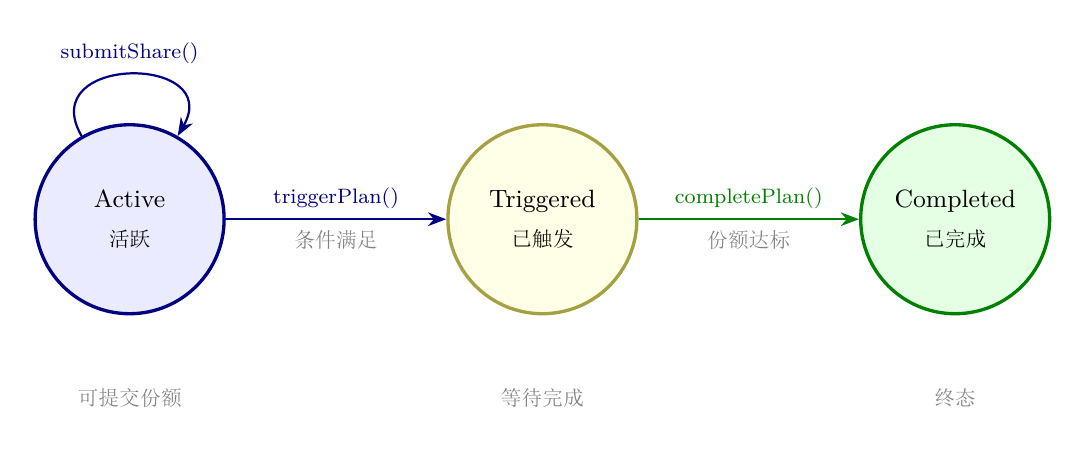
\includegraphics[width=1.0\textwidth]{figures/fig_statemachine.png}
\caption{智能合约状态机：单向状态转换 Active $\to$ Triggered $\to$ Completed}
\label{fig:statemachine}
\end{figure}

合约安全设计涵盖四个层面：权限控制（onlyOwner/onlyGuardian修饰符的require检查）、状态完整性（每函数入口require当前状态合法性）、输入校验（guardianAddresses长度、commitments长度、threshold与totalShares的关系）和事件审计（PlanCreated、PlanTriggered、ShareSubmitted、PlanCompleted等indexed事件）。未来可从以下方向扩展：引入BLS门限签名实现链上密钥聚合；将Pedersen同态承诺材料提交至链上实现链上多项式一致性验证；采用UUPS代理模式支持合约逻辑迭代。


\section{AI助手、邮件通知与用户认证}

\subsection{AI助手双引擎架构}

为降低非专业用户配置门限密码学参数的门槛，系统设计了AI助手模块，采用\textbf{规则引擎 + 大语言模型（LLM）双引擎架构}，根据API密钥配置情况自动选择工作模式。

\noindent\textbf{规则引擎模式（本地优先）。}当未配置LLM API密钥时，系统使用基于正则表达式的规则匹配引擎（aiService.ts）。该引擎定义了14种意图类型，覆盖遗产计划全生命周期的核心操作：

\begin{table}[H]
\centering
\caption{AI助手意图类型定义}
\label{tab:ai_intents}
\begin{tabularx}{\textwidth}{p{2.8cm}p{2.8cm}X}
\toprule
意图类型 & 意图标识 & 触发示例\\
\midrule
创建计划 & create\_plan & "创建遗产计划"、"发起遗产"\\
继承计划 & inherit\_plan & "继承计划ID xxx"、"申请继承"\\
提交份额 & submit\_share & "提交份额"、"确认份额"\\
添加资产 & add\_asset & "添加资产：比特币"\\
添加监护人 & add\_guardian & "添加监护人张三"\\
设置门限 & set\_threshold & "设置门限为2-of-3"\\
设置时间锁 & set\_timelock & "设置时间锁为30天"\\
查询计划 & query\_plans & "查看我的计划"\\
查询状态 & query\_status & "查询计划状态"\\
帮助 & help & "帮助"、"能做什么"\\
\bottomrule
\end{tabularx}
\end{table}

每条意图规则包含正则模式数组（patterns）、参数提取器数组（paramExtractors）和示例列表（examples）。参数提取器支持多种中文自然语言表达变体，例如计划ID可通过中文冒号分隔、UUID格式正则 \texttt{[a-f0-9\textbackslash-]\{36\}} 和英文冒号分隔等多种方式提取。置信度计算综合考虑模式匹配率（权重0.5）、参数提取成功率（权重0.3）和输入长度与示例平均长度的匹配度（权重0.2）。

\noindent\textbf{LLM模式（云端增强）。}当配置Deepseek API密钥后，系统切换至LLM驱动模式（llmService.ts）。该模式通过结构化系统提示词（system prompt，约1200字符）向LLM注入项目领域知识，使模型理解遗产计划创建、份额提交、状态查询等操作的业务语义和参数约束。系统提示词涵盖可用工具列表、调用格式规范（JSON格式的tool/args结构）、参数完整性规则以及四项重要约束：（1）创建计划时必须主动询问时间锁配置；（2）总份额数自动等于监护人数量；（3）监护人必须是系统注册用户；（4）文件资产通过上传功能添加并自动合并。

LLM以JSON格式返回工具调用指令，后端通过括号匹配算法（extractJsonObjects方法）从模型响应中提取JSON对象，解析tool和args字段，调用对应的executeTool方法执行业务逻辑，最后将结构化结果格式化为用户友好的文本返回。工具执行层面的关键安全设计包括监护人邮箱注册验证和监护人身份的双重匹配（用户ID + 邮箱）。

LLM模式相比规则引擎具有以下优势：（1）理解非固定模式的自然语言表达，不依赖预定义的正则模板；（2）支持多轮对话的上下文关联，例如用户先提"创建计划"再补充"名字叫我的遗产"，模型能正确关联前后信息；（3）主动引导用户补全缺失参数，例如创建计划时自动询问是否设置时间锁。

\noindent\textbf{降级策略。}当LLM API调用失败或未配置密钥时，系统自动回退至规则引擎模式，保证AI助手的基础可用性。这种双引擎设计遵循"优雅降级"原则，确保了系统在不同部署条件下的功能连续性。

\subsection{对话上下文状态机}

AI助手维护一个会话级的状态机（DialogContext / LLMContext），跟踪用户当前所处的操作阶段和已收集的信息。状态机包含以下核心字段：

\begin{itemize}
\item \textbf{currentStep}：当前操作阶段，取值范围为 \texttt{idle}（空闲）、\texttt{creating}（创建中）、\texttt{inherit}（继承中）、\texttt{submitting}（提交中）。
\item \textbf{workingPlan}：当前正在构建的计划对象，渐进式填充名称、资产、监护人、门限和时间锁等字段。规则引擎模式下直接在内存中维护；LLM模式下通过上下文消息传递给模型。
\item \textbf{collectedData}：已收集的散列数据，用于跟踪缺失参数。
\item \textbf{history / messages}：对话历史记录。规则引擎使用简化的 \texttt{role+content} 数组；LLM模式使用完整的OpenAI格式消息列表，支持 \texttt{system/user/assistant/tool} 四种角色。
\end{itemize}

状态机使得AI助手能够实现\textbf{多轮渐进式引导}。以创建计划为例，引擎首先检查workingPlan是否已初始化（未初始化则创建空计划并进入creating状态），然后逐项检查名称、资产、监护人是否已填充，每次返回针对性的引导提示。当资产和监护人收集完毕后，增设timeLockPrompted标志并询问用户是否需要设置时间锁。所有信息收集齐全后，进行监护人注册验证，通过后调用createPlan完成创建。规则引擎模式下由handleCreatePlan方法显式管理状态转移链；LLM模式下由系统提示词中的约束规则驱动模型行为，工具调用结果反馈至对话上下文形成闭环。

\subsection{LLM工具调用与Function Calling}

LLM模式下，系统实现了类OpenAI Function Calling的工具调用机制。后端向Deepseek API发送请求时注入包含9个工具定义的完整schema（createPlan、addAsset、addGuardian、setThreshold、setTimeLock、inheritPlan、submitShare、queryPlans、queryStatus），每个工具定义包含参数名称、类型、是否必填和中文描述。

模型在理解用户意图后，以JSON格式返回工具调用指令：\texttt{\{"tool":"createPlan","args":\{...\}\}}。后端通过括号匹配算法提取JSON对象，支持单次响应中的多个工具调用（依次执行并合并结果）。工具执行后，结构化结果（success/message/data）被解析为自然语言文本返回用户。

工具执行层面的关键设计：
\begin{itemize}
\item \textbf{监护人注册验证}：createPlan和addGuardian工具在执行前通过userService.getUserByEmail验证邮箱是否已注册，拒绝向非系统用户分发份额。
\item \textbf{文件资产合并}：LLM上下文中暂存的临时文件资产（通过界面上传的加密文件）在创建计划时自动合并到资产列表，无需用户重复添加。
\item \textbf{监护人身份匹配}：submitShare工具通过用户ID和邮箱双重匹配确定监护人身份——先尝试ID直接匹配，失败后通过邮箱查找对应监护人，适应不同命名约定的场景。
\item \textbf{参数完整性检查}：submitShare在执行前检查planId和shareValue是否为空，为空时返回明确的参数缺失提示而非静默失败。
\end{itemize}

\subsection{临时文件管理}

LLM服务内置了临时文件存储机制，支持用户通过AI助手界面直接上传文件作为加密资产。上传的文件以Base64编码存储在服务端内存Map中（key为临时文件ID，value含文件名、类型、大小和内容），并设置1小时自动过期清理（setTimeout调用Map.delete）。文件上传后通过系统消息（role: system）通知LLM文件已添加及文件元信息，模型在后续创建计划时自动将其合并至资产列表。

\subsection{命令执行与意图处理}

规则引擎模式下，executeCommand方法根据解析出的意图类型分发到对应的专用处理函数。各处理函数在统一的DialogContext上操作，保证了状态的一致性和可追踪性：

\begin{itemize}
\item \textbf{handleCreatePlan}：管理七步状态转移链（检查workingPlan $\to$ 收集名称 $\to$ 收集资产 $\to$ 收集监护人 $\to$ 询问时间锁 $\to$ 验证监护人注册 $\to$ 调用createPlan），每步返回针对性的引导文本。
\item \textbf{handleAddAsset}：文件类型资产检测（重定向至文件上传功能），非文件资产追加至workingPlan.assets并展示更新后的资产列表。
\item \textbf{handleAddGuardian}：验证监护人邮箱注册状态，自动更新totalShares（等于监护人数量），确保threshold不超过totalShares。
\item \textbf{handleQueryPlans}：按角色分类展示计划（创建的计划、继承的计划、监护的计划），无计划时引导用户创建。
\item \textbf{handleHelp}：返回分类的功能说明文本，涵盖创建、继承、监护和查询四类操作的示例指令。
\item \textbf{handleUnknown}：友好提示加指令建议列表，降低用户在输入错误时的挫败感。
\end{itemize}

\subsection{前端AI助手界面}

前端AIAssistant组件（AIAssistant.tsx）实现为可展开的侧边栏对话框，支持文本输入和文件上传两种交互方式。输入区域采用固定定位的底部输入栏，消息列表自动滚动至最新消息。文件上传支持拖拽和点击选择，上传前进行客户端文件大小校验。对话界面区分用户消息和助手消息的视觉样式，助手消息支持多行格式化文本渲染。组件通过API服务层（api.ts）调用后端AI接口，文件上传首先通过临时文件存储接口上传至服务端，获取文件ID后在LLM消息中附带引用。

\begin{figure}[H]
\centering
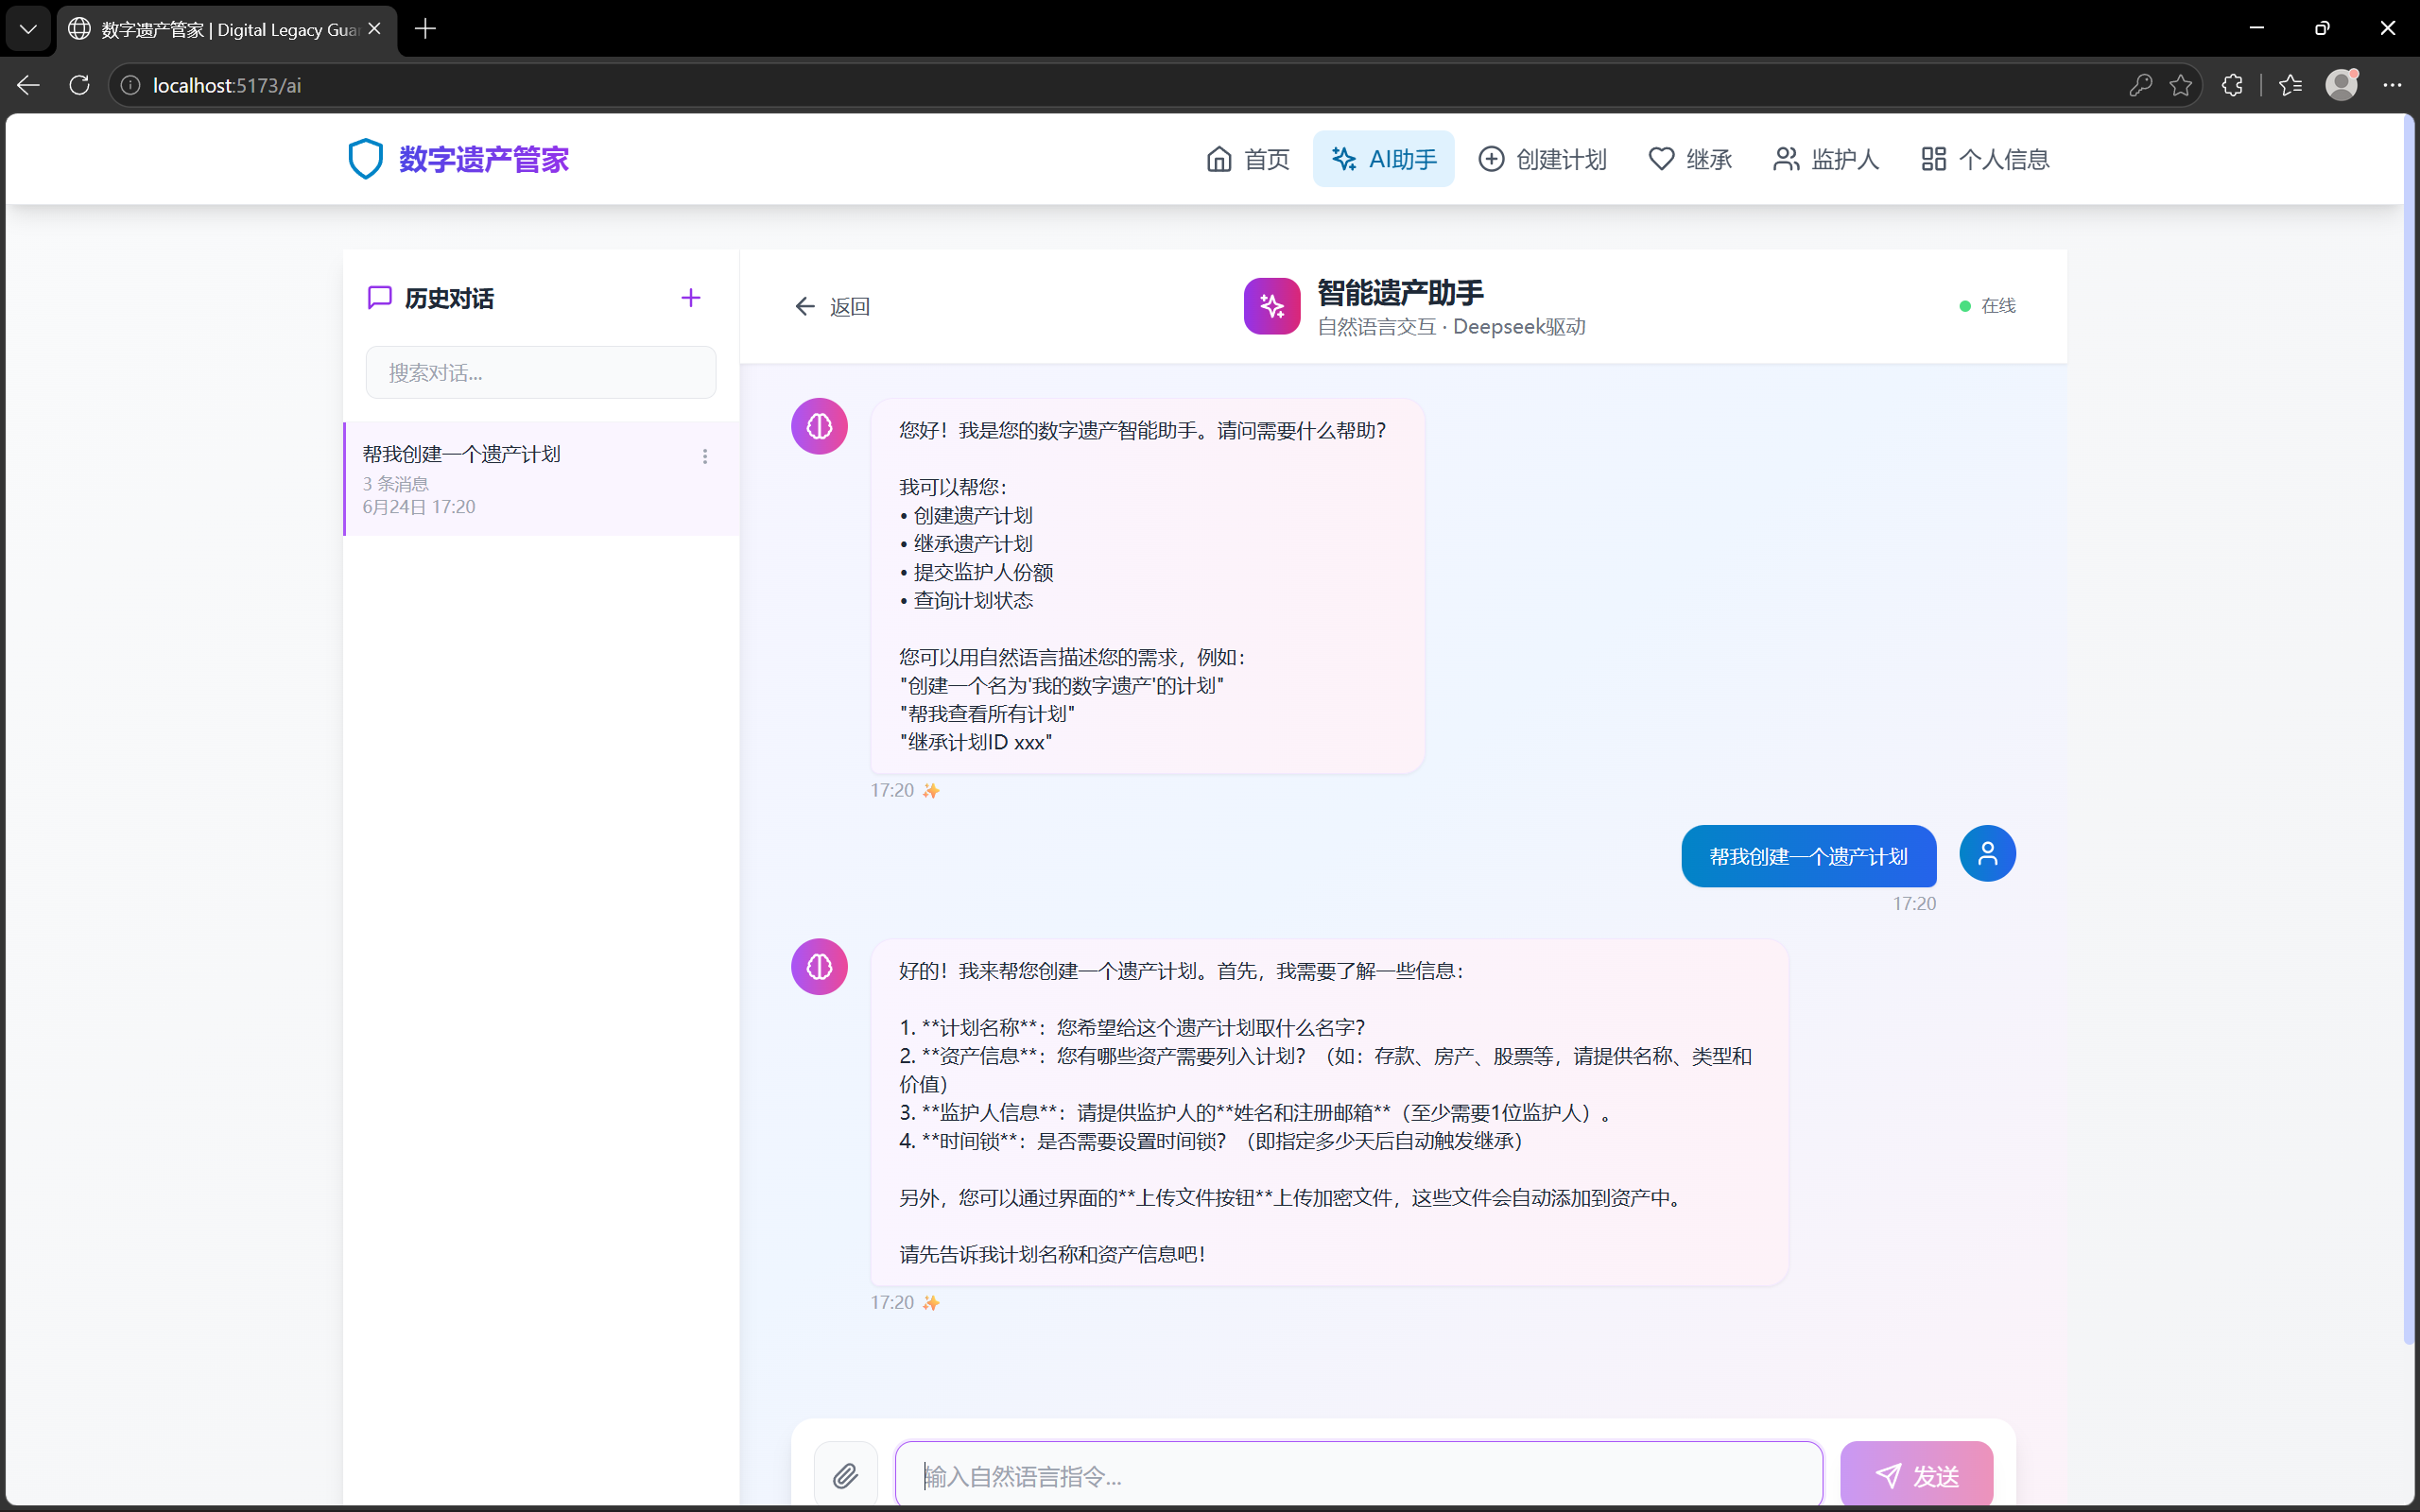
\includegraphics[width=1.0\textwidth]{figures/screenshots/AI助手对话页面.png}
\caption{AI助手对话页面——支持自然语言交互式操作与文件上传}
\label{fig:ss_ai}
\end{figure}

\subsection{邮件通知}

系统在五个关键事件触发邮件通知：份额分发（创建后立即向监护人发送含份额明文的邮件——这也是份额明文通过外部渠道传输的唯一时机）、继承发起广播、份额提交确认、继承完成通知（含解密资产列表）和登录验证码。邮件服务封装了Nodemailer SMTP发送，支持HTML格式邮件，竞赛演示模式下输出到控制台日志。

\begin{figure}[H]
\centering
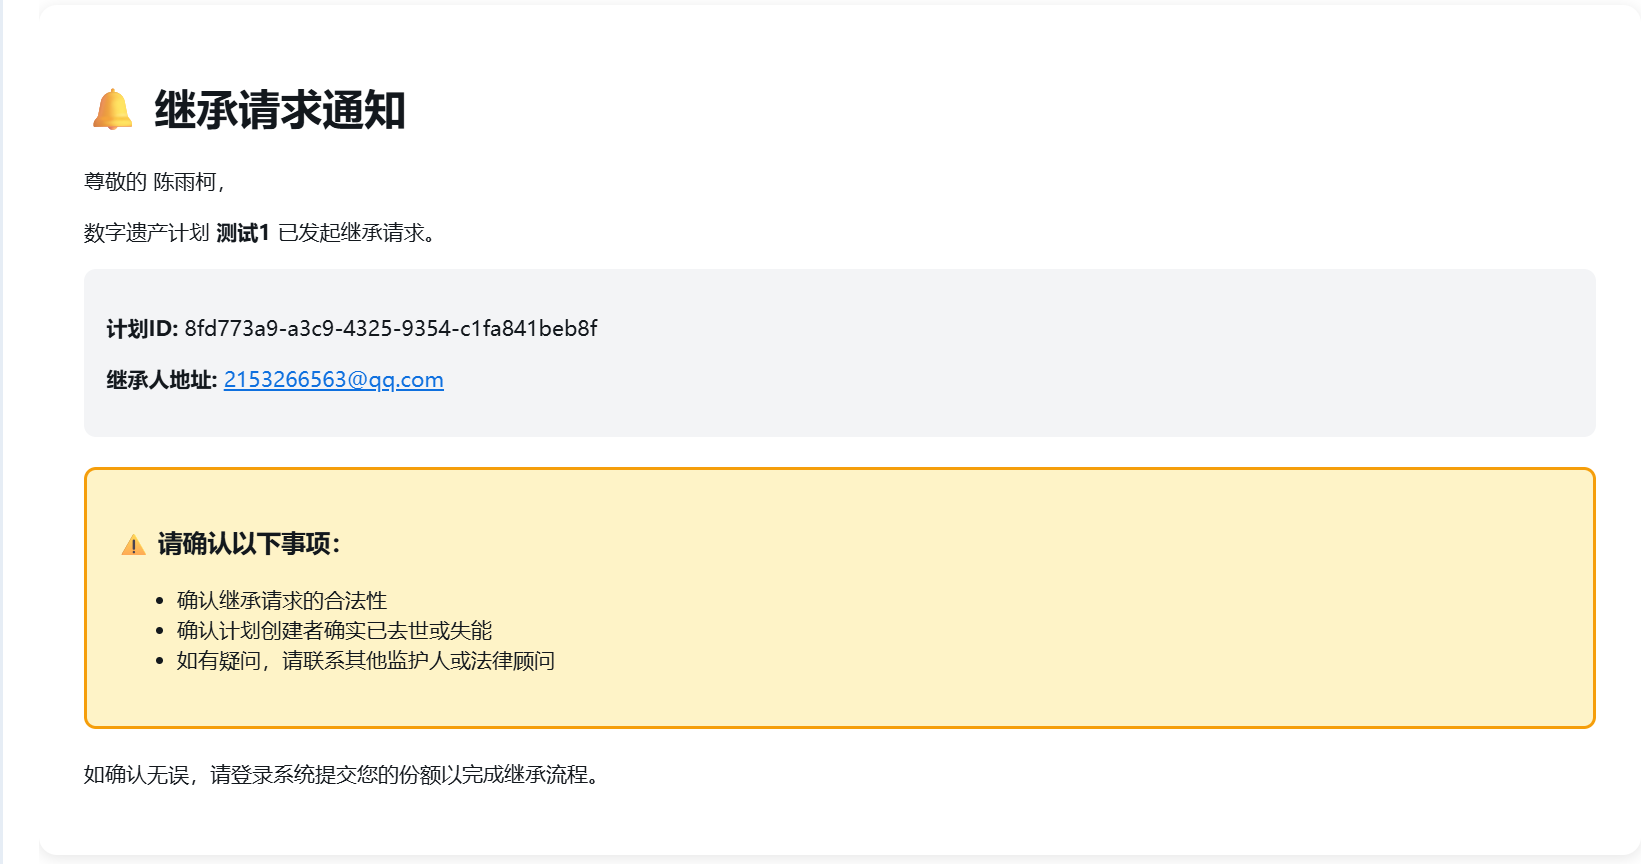
\includegraphics[width=1.0\textwidth]{figures/screenshots/邮件通知1.png}
\caption{邮件通知——份额分发邮件示例}
\label{fig:ss_email1}
\end{figure}

邮件服务的设计遵循以下安全原则：（1）份额明文仅在创建时通过邮件发送一次，后端不保存副本；（2）邮件内容不含主密钥——主密钥在创建时即被拆分且自身被丢弃；（3）继承完成邮件中的解密资产列表直接发送给继承人邮箱，不在服务端持久化解密结果。

\subsection{用户认证}

用户认证系统采用PBKDF2-SHA512密码哈希存储方案（16字节随机盐值，10000次迭代），用户ID为4位字母数字随机生成。登录验证码通过邮件发送，有效期为5分钟。认证模块独立于业务逻辑，用户密码的哈希值不参与密码学运算（密钥生成使用独立的随机源），确保认证系统与密码学系统之间的安全隔离。




% ==================== 第三章 作品测试与分析 ====================
\chapter{作品测试与分析}

\section{测试策略与概述}

测试环境基于Windows 11 + Node.js 18+，密码学库使用elliptic (secp256k1)和crypto-js (AES/SHA256)，合约测试使用Solidity 0.8.19 + Hardhat + ethers.js + Chai，存储为本地JSON文件，邮件为控制台输出模拟模式。

测试按照\textbf{单元测试（密码学模块）$\to$ 接口测试（API端点）$\to$ 安全测试（篡改和异常路径）$\to$ 合约测试（Solidity状态机）$\to$ 端到端演示验证}五个层次递进组织。底层关注密码学算法的数学正确性，中层验证API接口的参数校验和业务流程，上层通过攻击模拟和端到端场景验证系统的整体安全防护能力。

\begin{figure}[H]
\centering
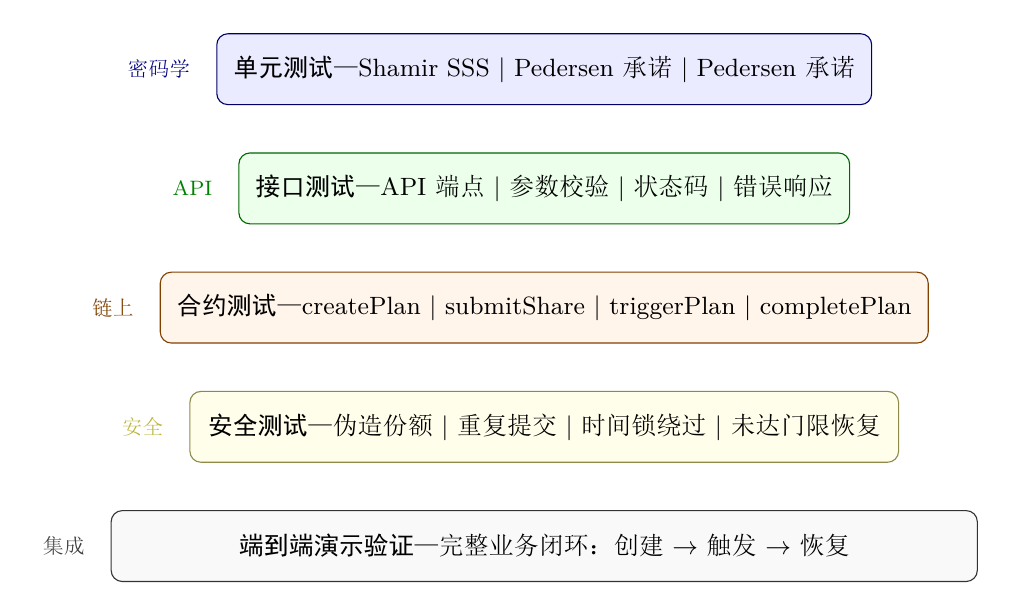
\includegraphics[width=1.0\textwidth]{figures/fig_testpyramid.png}
\caption{测试金字塔：底层密码学单元测试为数学正确性兜底，逐层向上扩展至端到端演示验证，覆盖广度递增而测试数量递减}
\label{fig:testpyramid}
\end{figure}

\section{核心测试用例}

以下按三组列出核心测试用例，略去用户注册登录等基础 CRUD 操作和辅助功能用例，仅保留对安全性有直接验证作用的测试项。

\setlength{\extrarowheight}{3pt}
\begin{longtable}{p{2.5cm}p{3.8cm}p{3.8cm}p{4.5cm}}
\caption{核心测试用例}\\
\toprule
编号 & 验证场景 & 测试操作 & 期望结果\\
\midrule
\endfirsthead
\toprule
编号 & 验证场景 & 测试操作 & 期望结果\\
\midrule
\endhead
\multicolumn{4}{l}{\textbf{计划管理与参数校验（T01--T05）}}\\
\midrule
T01 & 计划创建正确性 & 创建完整计划参数 & 返回 active 状态，shares 不含 value\\
T02 & 门限超范围 & threshold $>$ totalShares & 创建被拒绝，提示超范围\\
T03 & 份额数超监护人 & totalShares $>$ guardians.length & 创建被拒绝\\
T04 & 空资产创建 & assets = [ ] & 创建被拒绝\\
T05 & 份额不持久化 & 查询已创建计划 & shares 仅含承诺值，不含 value\\
\midrule
\multicolumn{4}{l}{\textbf{继承流程与安全验证（T06--T15）}}\\
\midrule
T06 & 共识触发继承 & 发起继承请求 & 计划变更为 collecting\\
T07 & 时间锁未到期 & timed 模式下提前触发 & 被拒绝，返回精确剩余时间\\
T08 & 时间锁到期 & timed 模式到期触发 & 正常进入 collecting\\
T09 & 正确份额提交 & 提交正确 shareValue & 计数 +1，标记已提交\\
T10 & 份额字符篡改 & 修改一个十六进制字符 & Pedersen 验证立即拒绝\\
T11 & 随机字符串提交 & 非十六进制随机值 & 格式校验 + 承诺验证双拒绝\\
T12 & 重复提交 & 同一监护人再次提交 & 拒绝，计数不增加\\
T13 & 非监护人提交 & 不在列表中的 ID & 返回 "Guardian not found"\\
T14 & 未达门限恢复 & 有效份额 $<$ threshold & 信息论层面拒绝\\
T15 & 达门限恢复 & 有效份额 $\ge$ threshold & Lagrange 恢复 + AES 解密 + completed\\
\midrule
\multicolumn{4}{l}{\textbf{智能合约状态机测试（T16--T26）}}\\
\midrule
T16 & 合约创建计划 & createPlan 有效参数 & 触发 PlanCreated 事件\\
T17 & 合约非法参数 & threshold $>$ totalShares & revert\\
T18 & 合约重复 planId & 相同 planId 再次创建 & revert\\
T19 & 合约提交份额 & guardian 调用 submitShare & ShareSubmitted 事件，hasSubmitted=true\\
T20 & 合约非监护人提交 & owner 调用 submitShare & onlyGuardian 修饰符 revert\\
T21 & 合约重复提交 & 同一 guardian 再次提交 & revert\\
T22 & 合约时间锁到期触发 & evm\_increaseTime + triggerPlan & PlanTriggered 事件\\
T23 & 合约时间锁未到期 & 直接 triggerPlan & revert\\
T24 & 合约完成计划 & 达门限 completePlan & 状态变更为 Completed\\
T25 & 合约未触发完成 & Active 状态 completePlan & revert\\
T26 & 合约查询 & getPlan / getGuardianInfo & 返回数据与创建一致\\
\bottomrule
\end{longtable}

上述 26 条用例完整覆盖了系统的三条关键路径：正常创建与继承（T01、T06、T08、T09、T15）验证了门限密码学方案在Web应用中的端到端可行性；安全异常路径（T02--T05、T07、T10--T14）验证了参数校验、承诺验证、时间锁和防重机制在逆向输入下的正确拒绝行为；合约状态机路径（T16--T26）验证了链上状态转换约束和权限控制逻辑。

\section{密码学功能正确性验证}
\label{sec:crypto_correctness}

在安全性分析之前，首先验证密码学核心算法的数学正确性——确保Shamir秘密共享的拆分与恢复、Pedersen承诺的同态性质以及零和多项式刷新在实现层面没有引入错误。

\subsection{Shamir秘密共享正确性}

为验证Shamir秘密共享实现的正确性，在$n \in \{3, 5, 7, 10\}$、$t \in \{2, 3, 5, 7\}$的参数组合下各进行100轮随机测试。测试流程：随机生成256位主密钥$\to$使用$t$-of-$n$拆分$\to$随机选取$t$个份额$\to$Lagrange插值恢复$\to$与原始主密钥对比。

\begin{table}[H]
\centering
\caption{Shamir正确性验证结果}
\label{tab:shamir_test}
\begin{tabularx}{\textwidth}{cccccc}
\toprule
$n$ & $t$ & 测试轮数 & 成功次数 & 正确率 & 平均耗时(ms)\\
\midrule
3 & 2 & 100 & 100 & 100.00\% & 0.0101\\
5 & 3 & 100 & 100 & 100.00\% & 0.0123\\
7 & 5 & 100 & 100 & 100.00\% & 0.0629\\
10 & 7 & 100 & 100 & 100.00\% & 0.0406\\
\bottomrule
\end{tabularx}
\end{table}

全部参数组合的正确率均为100.00\%，验证了Shamir拆分与Lagrange恢复在secp256k1标量域$\mathbb{F}_q$上的实现正确性。

\subsection{同态刷新正确性验证}

验证刷新后的份额使用Lagrange插值恢复的主密钥与原始主密钥一致。每项参数进行100轮测试。刷新流程：生成主密钥$\to$拆分得到$v_i,r_i$$\to$生成零和多项式$Z_v(x),Z_r(x)$$\to$计算新份额$v'_i = v_i + Z_v(i)$$\to$用$t$个$v'_i$恢复$s'$$\to$验证$s' = s$。

\begin{table}[H]
\centering
\caption{同态刷新正确性验证结果}
\label{tab:refresh_test}
\begin{tabularx}{\textwidth}{cccccc}
\toprule
$n$ & $t$ & 测试轮数 & 刷新前正确率 & 刷新后正确率 & 刷新耗时(ms)\\
\midrule
3 & 2 & 100 & 100.00\% & 100.00\% & 0.0304\\
5 & 3 & 100 & 100.00\% & 100.00\% & 0.0671\\
7 & 5 & 100 & 100.00\% & 100.00\% & 0.1746\\
10 & 7 & 100 & 100.00\% & 100.00\% & 0.2480\\
\bottomrule
\end{tabularx}
\end{table}

刷新前后正确率均为100.00\%，且主承诺$C_{\text{master}}$保持不变（$Z_v(0)=Z_r(0)=0$），验证了零和多项式方法的数学正确性。

\subsection{主承诺同态验证精度测试}

测试主承诺同态验证$\Sigma(\lambda_j \cdot C_{i_j}) = C_{\text{master}}$的精度。正确份额应通过验证，错误份额（随机值）应被拒绝。100轮测试结果如下：

\begin{table}[H]
\centering
\caption{同态验证精度测试}
\label{tab:verify}
\begin{tabularx}{\textwidth}{lccccc}
\toprule
指标 & TP & FN & FP & TN & Accuracy\\
\midrule
综合（100轮） & 100 & 0 & 0 & 100 & 100.00\%\\
\bottomrule
\end{tabularx}
\end{table}

零假阳性和零假阴性结果表明，同态验证机制能够以密码学强度精确区分正确份额与伪造份额。

\section{智能合约测试}

合约测试使用Hardhat测试框架配合Chai断言库和ethers.js，是项目中唯一拥有自动化测试代码的模块（文件位于\texttt{contracts/test/LegacyContract.test.js}）。测试覆盖计划创建、份额提交和计划触发三个describe块，对应T16--T26共11个测试用例。正常路径测试验证了PlanCreated事件触发、时间锁到期后PlanTriggered事件触发以及达门限后PlanCompleted事件触发；异常路径测试验证了非法参数revert、重复planId拒绝、非监护人提交拒绝、重复提交拒绝、时间锁未到触发拒绝和未触发状态完成拒绝。测试利用Hardhat内置网络的\texttt{evm\_increaseTime}方法模拟时间流逝，高效验证了时间锁机制的正确性。

\section{性能测试与分析}
\label{sec:performance}

\subsection{密码学操作性能基准}

各操作在预热后测试200轮取平均。实验环境：Intel i7-12800HX (24核) / 15.75GB RAM / Node.js v20.19.4。

\begin{table}[H]
\centering
\caption{密码学操作性能基准}
\label{tab:perf_bench}
\begin{tabularx}{\textwidth}{lc}
\toprule
操作 & 平均耗时(ms)\\
\midrule
主密钥生成（256-bit） & 0.0206\\
Pedersen双多项式拆分（5-of-3） & 0.0940\\
Pedersen承诺生成 & 1.3569\\
Pedersen承诺验证 & 1.2574\\
零和多项式增量生成（5份） & 0.0693\\
承诺同态刷新计算（5份） & 6.8089\\
Lagrange恢复主密钥（3份） & 0.0054\\
主承诺同态验证（3份） & 1.6624\\
ECIES加密 & 1.5716\\
ECIES解密 & 0.9351\\
\bottomrule
\end{tabularx}
\end{table}

所有密码学操作均在毫秒级完成。最耗时的承诺同态刷新计算（6.81ms）涉及5次独立EC点加法，但该操作为离线刷新场景，不影响用户交互的响应时间。

\subsection{规模扩展性测试}

不同监护人数目$n$和门限$t$下各操作耗时（50轮取平均）：

\begin{table}[H]
\centering
\caption{规模扩展性测试}
\label{tab:scalability}
\begin{tabularx}{\textwidth}{cccc}
\toprule
$(n, t)$ & 拆分耗时(ms) & 刷新耗时(ms) & 恢复耗时(ms)\\
\midrule
(3, 2) & 0.054 & 0.034 & 0.004\\
(5, 3) & 0.098 & 0.125 & 0.007\\
(7, 5) & 0.175 & 0.154 & 0.016\\
(10, 7) & 0.299 & 0.239 & 0.032\\
\bottomrule
\end{tabularx}
\end{table}

各操作耗时随$(n,t)$增长呈温和的$O(nt)$趋势，在典型配置（3-of-5或5-of-9）下的响应时间均在100ms以内，完全满足竞赛演示的交互需求。

\subsection{计算开销分布}

密码学计算主要涵盖以下操作的理论复杂度：\textbf{主密钥生成}使用拒绝采样在 secp256k1 标量域中生成随机标量，期望 $O(1)$ 时间，每次采样消耗 32 字节随机数，期望拒绝次数约为 1。\textbf{秘密共享拆分}的计算量集中在 $n$ 次多项式求值、$n$ 次 EC 乘法和 $(t-1)$ 次 EC 乘法，总体复杂度 $O(nt)$，其中多项式求值使用快速幂 $O(\log t)$，EC 乘法使用 double-and-add 算法。\textbf{份额验证}的核心是主承诺同态聚合验证，对每个份额执行 Lagrange 系数标量乘加，复杂度 $O(t)$。\textbf{拉格朗日插值}恢复需要 $t^2$ 次模乘和 $t$ 次模逆运算，复杂度 $O(t^2)$。\textbf{AES 加解密}使用 AES-256-CBC，复杂度与明文大小 $|M|$ 线性相关，资产包通常在 KB 级别，开销极低。

\begin{figure}[H]
\centering
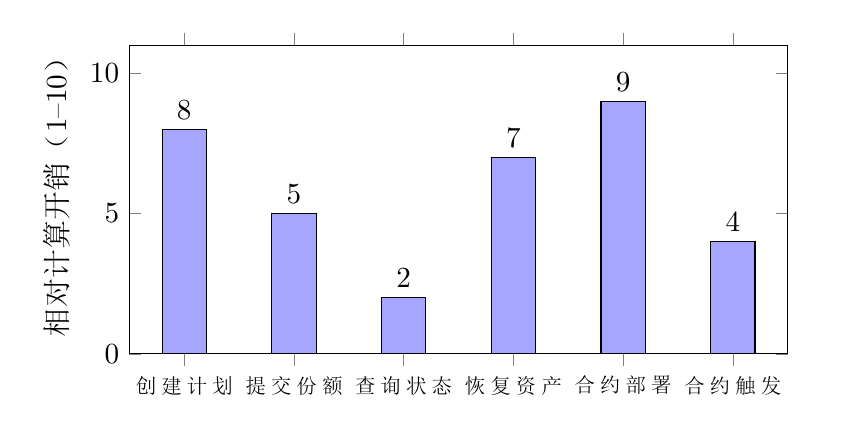
\includegraphics[width=1.0\textwidth]{figures/fig_perf_chart.png}
\caption{主要操作相对计算开销估计：EC点运算主导了承诺生成和刷新操作，多项式运算和AES加解密开销极低}
\label{fig:perf_chart}
\end{figure}

在实际门限参数配置下（通常为3-of-5或5-of-9），创建计划和提交份额的EC运算次数分别为约7次和约6次，单次接口响应时间在100ms以内。

\subsection{工程化考量}

当前原型使用本地JSON文件存储（每计划约2--5KB），适合竞赛演示和小规模验证。生产环境可将JSON替换为PostgreSQL，加密资产包迁移至IPFS/对象存储。原型在localhost环境运行未启用TLS，生产部署应启用HTTPS和S/MIME端到端邮件加密。系统在以下方面存在改进空间：元信息字段级加密防止社会关系网络泄露；盲签名技术使服务器在不了解监护人身份的情况下验证份额；渐进式解密机制防止继承人设备被盗后资产直接暴露。智能合约层面需关注重入攻击（当前采用checks-effects-interactions模式缓解）、前端运行（commit-reveal方案）和gas消耗优化等问题。

\section{安全性分析}
\label{sec:security}

本节在确认密码学功能正确性（第\ref{sec:crypto_correctness}节）和性能可接受性（第\ref{sec:performance}节）的基础上，对系统的安全边界、威胁模型和攻击路径进行系统分析。

\subsection{密码学模块安全边界}

\subsubsection{随机数与秘密材料安全}

随机数生成使用Node.js的crypto.randomBytes（底层调用OS密码学安全随机源），通过拒绝采样保证有限域$\mathbb{F}_q$内均匀分布。系统中三类核心秘密材料——主密钥$K$（仅存在于createPlan的局部变量，拆分后不再被引用）、多项式系数$a_1,\dots,a_{t-1}$（仅存在于split局部数组）、份额值$y_1,\dots,y_n$（仅通过邮件发送，不在后端持久化）——均遵循"即用即弃"原则，JavaScript GC将在函数返回后回收内存。

\subsubsection{椭圆曲线运算正确性与代码质量}

EC运算使用elliptic库（经以太坊生态广泛审查），构造函数显式校验fieldOrder与groupOrder的一致性，确保Pedersen承诺的数学前提成立。模逆元使用扩展欧几里得算法（$O(\log q)$步内完成）。代码质量方面：TypeScript严格模式覆盖密码学模块；所有EC解码和模逆元运算由try-catch保护；模块无文件系统/网络依赖和全局状态，满足纯函数设计原则。

\subsection{威胁模型与防护矩阵}

本作品考虑的威胁模型包含以下攻击者类型及其能力假设：

\begin{enumerate}
  \item \textbf{外部攻击者：}可以读取服务器静态文件（plans.json、requests.json等），但无法获取监护人的电子邮件账户或份额邮件内容。
  \item \textbf{恶意监护人：}拥有自己的份额明文值，可能尝试伪造其他监护人的份额、重复提交自己的份额、或提交一个来自不同多项式实例的合法份额值。
  \item \textbf{恶意服务器管理员：}拥有数据库的完全读写权限，可以读取和修改所有JSON文件内容。
  \item \textbf{被动网络监听者：}可以截获前端与后端之间的HTTP通信（假设未启用HTTPS的场景）。
\end{enumerate}

\begin{table}[H]
\centering
\small
\caption{威胁模型与防护措施矩阵}
\setlength{\extrarowheight}{3pt}
\begin{tabularx}{\textwidth}{p{2.5cm}p{3.5cm}p{3.5cm}X}
\toprule
威胁 & 攻击方式 & 攻击者能力要求 & 防护设计\\
\midrule
单点泄露 & 监护人泄露份额 & 恶意监护人 & $<$门限$t$个份额无法恢复主密钥（信息论安全）。\\
伪造份额 & 提交篡改的shareValue & 任意攻击者 & Pedersen承诺验证，伪造在第一层即被拒绝（T10已证实）。\\
跨计划注入 & 将A计划的份额提交到B计划 & 持有他计划份额的监护人 & 承诺绑定到特定多项式，不同计划的系数不同，验证必然失败。\\
份额重用 & 从公开存储获取$C_i$假装知道$v_i$ & 可访问plans.json & 提交时需用盲因子$r_i$重算承诺，攻击者不知$v_i$与$r_i$的匹配关系，无法通过单点验证。\\
提前继承 & 时间锁到期前发起继承 & 继承人 & 后端检查时间锁（T07已证实）；合约检查block.timestamp（T23已证实）。\\
重复提交 & 同一监护人多次提交 & 恶意监护人 & submittedGuardians数组防重（T12已证实）+hasSubmitted标志（T21已证实）。\\
服务器泄露 & 读取plans.json等文件 & 服务器权限攻击者 & StoredShare不含value（T05已证实）；encryptedAssets需主密钥解密；主密钥被门限拆分。\\
链上篡改 & 直接调用合约函数 & 以太坊账户攻击者 & require条件（T17已证实）、onlyGuardian修饰符（T20已证实）限制权限。\\
中间人攻击 & 拦截HTTP通信 & 网络监听者 & 份额通过邮件分发；CORS限制跨域；生产环境应启用HTTPS。\\
\bottomrule
\end{tabularx}
\end{table}

\subsection{安全属性的形式化表述与验证}

本系统的核心安全属性可以用如下形式化语言表述，每条属性在下文给出对应的测试验证：

\textbf{属性P1（份额保密性）：}对于任意攻击者$\mathcal{A}$，若其掌握的份额数量$m < t$，则$\mathcal{A}$关于主密钥$K$的优势为：
\[
\text{Adv}_{\mathcal{A}}^{\text{secrecy}} = \left|\Pr[\mathcal{A}(\text{Share}_{i_1},\dots,\text{Share}_{i_m}) = K] - \frac{1}{q}\right| = 0
\]
即攻击者无法以优于随机猜测的概率推断主密钥。这是Shamir秘密共享的信息论安全保证。\textbf{验证：}T05证实持久化存储中不含份额明文值，T14证实少于门限数量的份额无法触发恢复流程。

\textbf{属性P2（份额可验证性）：}对于任意提交的份额$(x_i', y_i')$，若$y_i' \neq f(x_i)$（其中$f$为原始多项式），则：
\[
\Pr[\text{Verify}(x_i', y_i') = \text{true}] \le \text{negl}(\lambda)
\]
即伪造份额通过验证的概率在安全参数$\lambda$下是可忽略的。这由Pedersen承诺在离散对数假设下保证。\textbf{验证：}T10证实修改shareValue中一个十六进制字符即被拒绝，T11证实随机字符串被格式校验和承诺验证双重拒绝，表\ref{tab:verify}的主承诺同态验证精度测试证实零假阳性。

\textbf{属性P3（恢复正确性）：}对于任意$t$个有效份额$\{(x_{i_j}, y_{i_j})\}_{j=1}^{t}$，拉格朗日插值恢复的秘密$S'$满足：
\[
S' = f(0) = K
\]
即正确恢复的秘密等于原始主密钥。这是拉格朗日插值在有限域上的代数正确性保证。\textbf{验证：}T15证实达到门限数量的有效份额能够正确恢复主密钥并成功解密资产，表\ref{tab:shamir_test}的多参数组合100轮测试进一步提供了统计验证。

此外，T07和T23分别从后端和合约两侧验证了时间锁保护的有效性，T12和T21分别从后端和合约两侧验证了防重复提交机制的可靠性。

\subsection{攻击路径分析}

针对四种攻击者角色，逐条推演可能的攻击路径和对应的防护阻断点：

\textbf{路径1——外部攻击者读取存储文件：}plans.json中shares使用StoredShare结构，仅保存承诺值和盲因子，不包含份额明文value字段（T05已证实）。encryptedAssets为AES-256密文，解密需要主密钥$K$。而$K$在创建计划后被Shamir拆分并丢弃，存储中不存在$K$的任何完整副本。攻击者仅读取存储文件无法恢复资产。

\textbf{路径2——恶意监护人伪造份额：}监护人Alice无法伪造Bob的份额。随机猜测$v'$提交时，系统使用Bob存储的盲因子$r_B$重算承诺$r_BG + v'H$，必然不等于$C_B$，第一层Pedersen单点验证立即拒绝（T10已证实）。即使Alice知晓Bob的盲因子$r_B$（可访问plans.json），也需要同时猜测正确的$v_B$值——$v_B$来源于256位有限域中的Shamir多项式求值，暴力猜测不可行。若Alice从另一个计划中窃取了合法份额$(v_A, r_A)$并提交至当前计划，由于当前计划存储的盲因子$r_B \neq r_A$，验证同样失败。跨计划份额注入进一步可被主承诺同态聚合验证检测——不同来源的份额集合无法通过$\sum \lambda_i C_i \stackrel{?}{=} C_{\text{master}}$的验证。

\textbf{路径3——继承人提前触发：}timed模式下，时间锁检查精确到秒级，提前触发的请求被拒绝并返回精确的剩余时间（T07已证实）。即使继承人绕过前端直接调用API，后端的Date对象毫秒级比较仍能拦截。consensus模式下继承请求虽可发起，但必须收集到$t$个监护人的有效份额（T14已证实），继承人本身不掌握任何份额值。合约侧triggerPlan检查block.timestamp（T23已证实），提前调用被require语句拒绝。

\textbf{路径4——恶意管理员修改状态：}攻击者即使获得plans.json的读写权限并修改计划状态为collecting，继承流程启动后仍需监护人提交有效份额值。份额明文仅在创建时通过邮件发送至监护人邮箱，服务端不保存副本。攻击者需同时攻破所有监护人的邮件账户才能获取足够份额；且在consensus模式下，监护人在收到不明继承通知后有动机主动核实，增加了攻击的暴露风险。

\subsection{密码学安全强度分析}

系统各组件的安全强度如下：

\begin{table}[H]
\centering
\small
\caption{密码学组件安全强度}
\setlength{\extrarowheight}{3pt}
\begin{tabularx}{\textwidth}{p{3cm}p{2.2cm}p{2.8cm}X}
\toprule
密码学组件 & 安全级别 & 基础假设 & 攻击代价\\
\midrule
Shamir秘密共享 & 无条件安全（$m<t$） & 有限域多项式插值唯一性 & 枚举$q^{t-m}$个候选值，$q\approx 2^{256}$时不可行\\
AES-256加密 & 256位对称安全 & AES分组密码安全 & 暴力破解$2^{256}$次，量子Grover降至$2^{128}$\\
secp256k1 ECDLP & 128位非对称安全 & 椭圆曲线离散对数假设 & Pollard's rho需$2^{128}$步，量子Shor多项式时间求解（未实用化）\\
SHA256(Pedersen H点生成) & 128位原像安全 & 随机预言机模型 & 原像$2^{256}$\\
PBKDF2-SHA512 & $\sim$200位口令安全 & 口令熵假设 & 复杂度$\approx$迭代次数$\times$哈希\\
\bottomrule
\end{tabularx}
\end{table}

需要注意的是，Shamir秘密共享的信息论安全属性是系统设计中的最强安全保障——无论攻击者拥有多少计算资源，只要没有收集到至少$t$个有效份额，从信息论角度就无法推断任何关于主密钥的信息。这一属性不依赖于任何计算复杂性假设（如离散对数假设），为长期数字遗产（可能跨越数十年）提供了超时间尺度的安全保证。

\section{前端界面演示验证}

前端基于React 18 + TypeScript构建，提供创建计划四步向导、控制台面板、继承流程、监护人门户和AI助手对话等页面。前端对门限参数实施双重校验（threshold $\ge$ 1、threshold $\le$ totalShares、totalShares $\le$ guardians.length），与后端校验形成安全防护闭环。以下为系统各核心页面的实际运行截图及功能说明。

\begin{figure}[H]
\centering
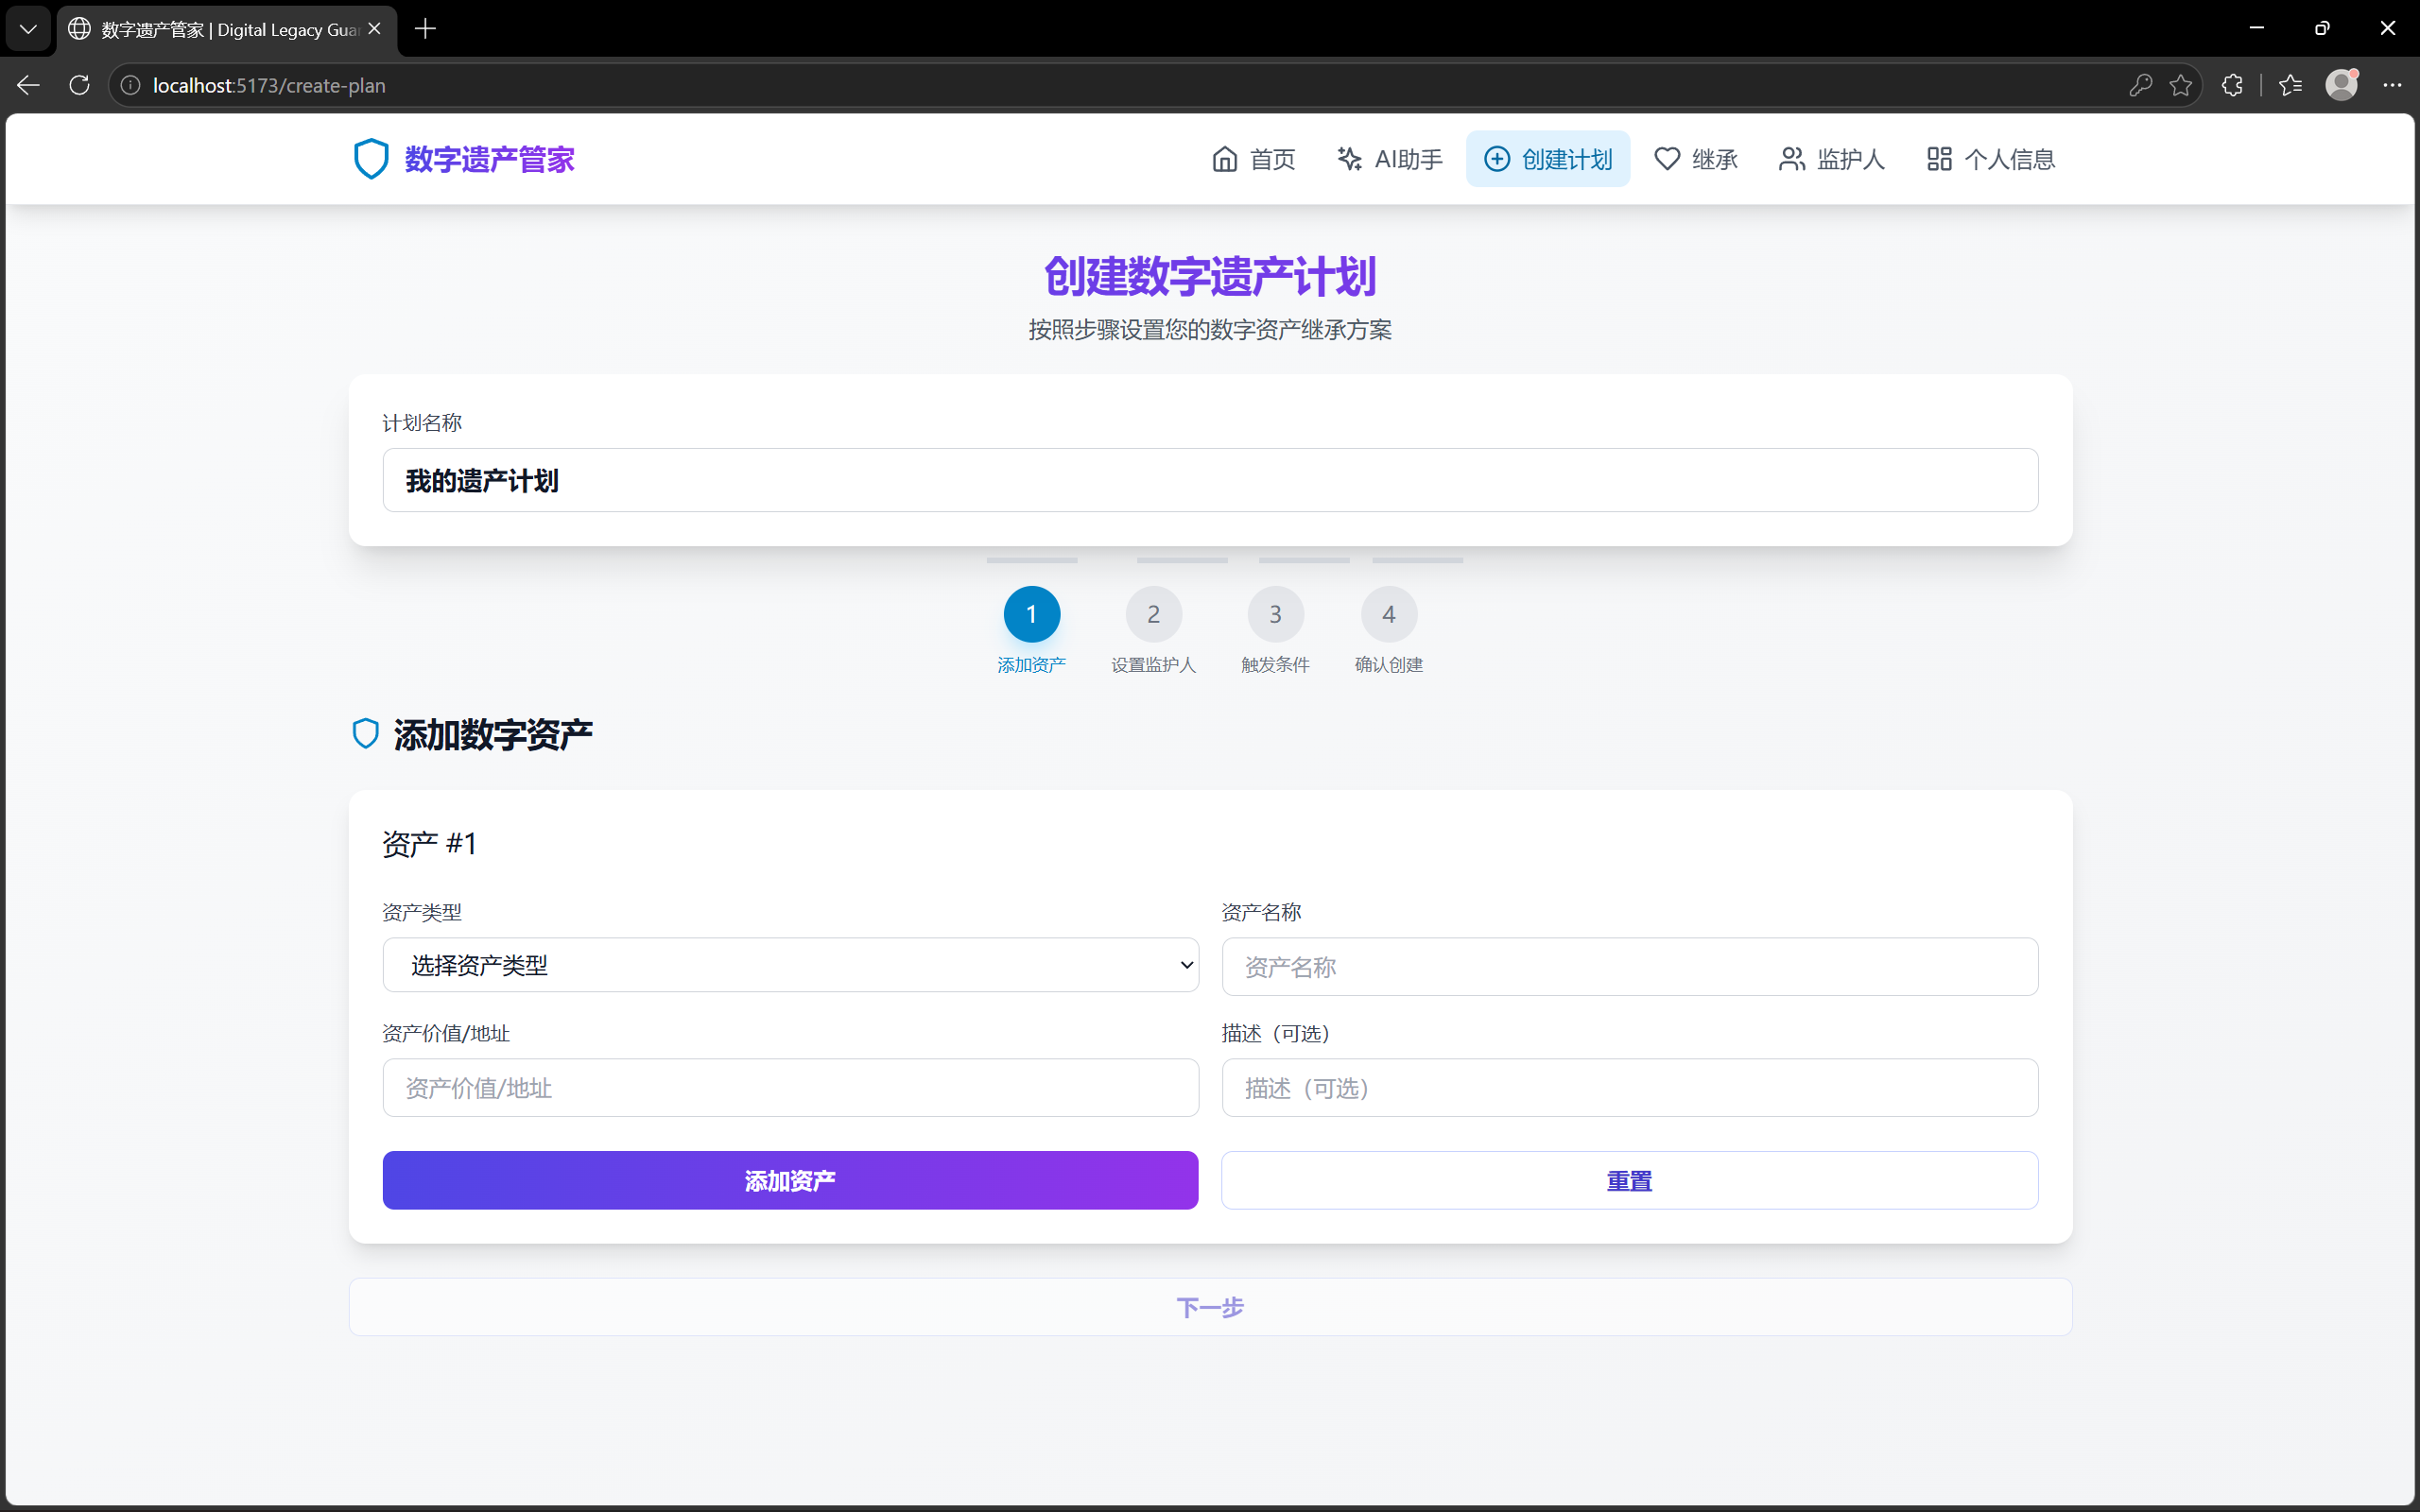
\includegraphics[width=1.0\textwidth]{figures/screenshots/创建遗产计划.png}
\caption{创建遗产计划页面——四步向导表单，依次引导用户完成资产添加（支持加密货币、云账号、加密文件、智能合约四种类型）、监护人选择（含用户搜索和自动填充）、触发条件配置（共识/时间锁模式）和最终确认，每步包含实时表单验证和中文错误提示}
\label{fig:ss_create}
\end{figure}

创建计划页面（图\ref{fig:ss_create}）采用四步向导设计，将门限密码学参数（$t$和$n$）的配置转化为分步引导式操作。用户在"设置监护人"步骤中通过搜索已注册用户添加监护人，系统自动计算$n$（总份额数）并实时展示$t$-of-$n$配置含义的文本解释，避免用户因不理解门限概念而设置不当参数。

\begin{figure}[H]
\centering
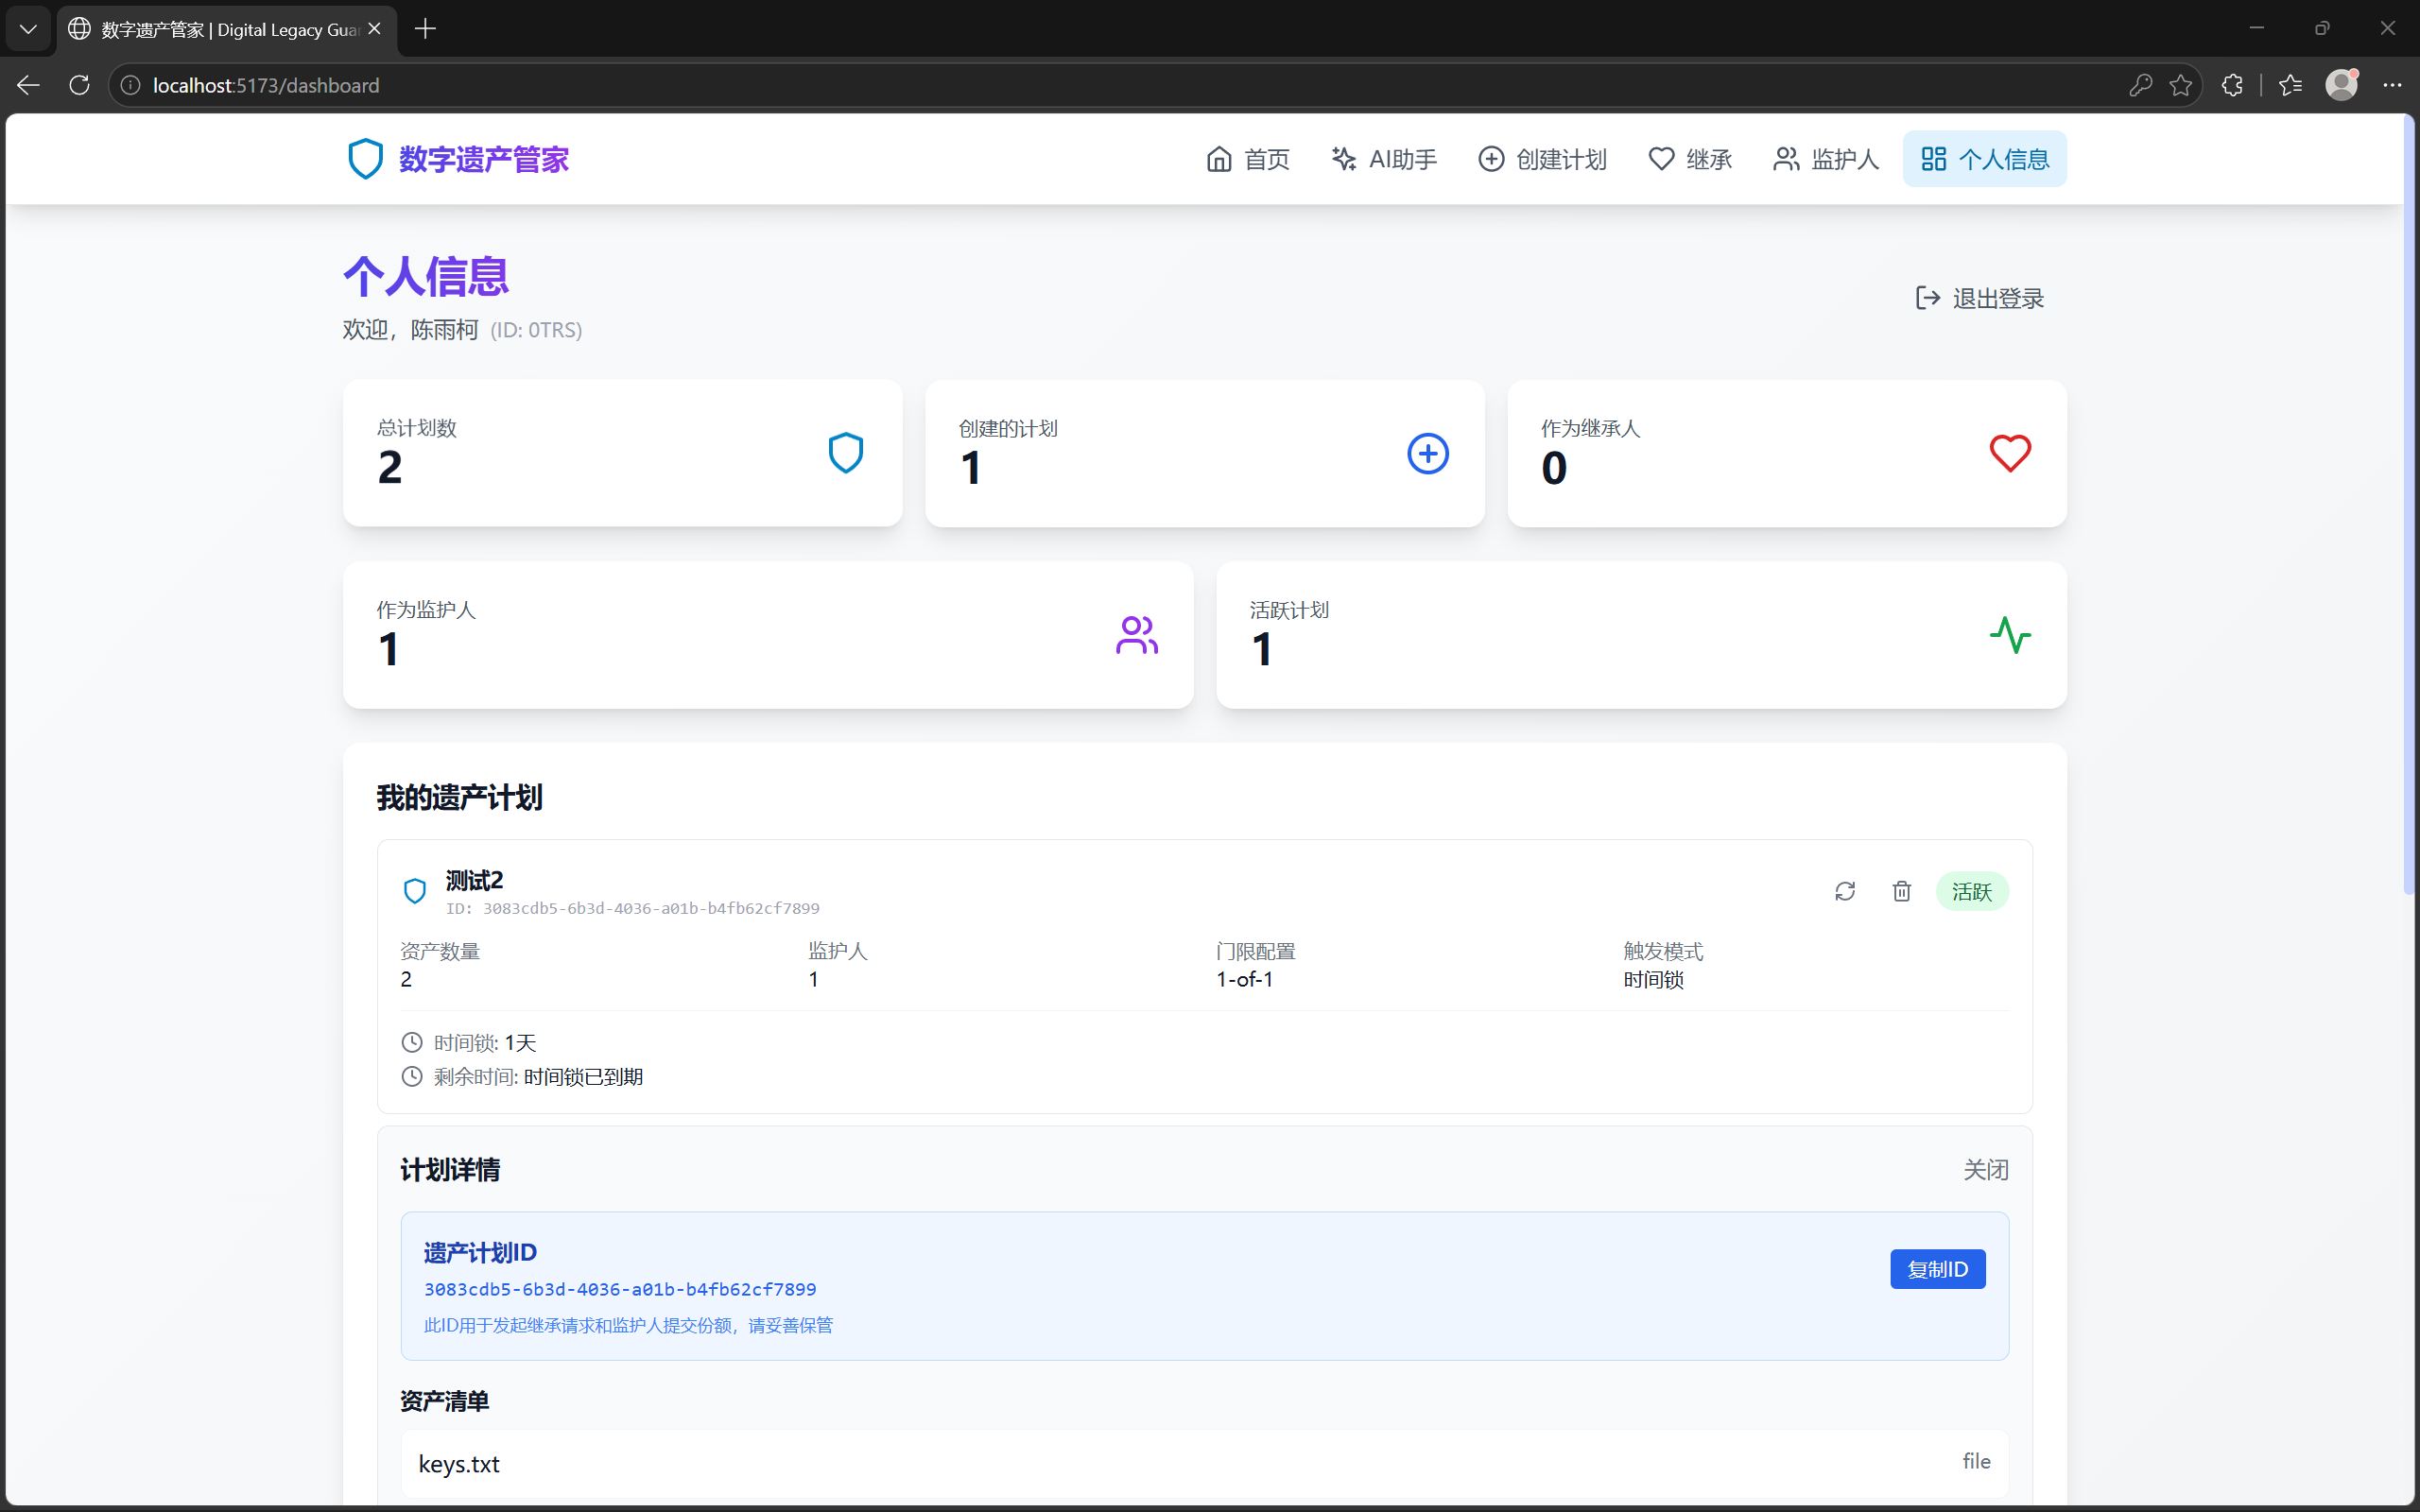
\includegraphics[width=1.0\textwidth]{figures/screenshots/控制台dashboard.png}
\caption{控制台Dashboard——遗产计划总览，按角色分类展示用户创建、继承和监护的计划，每项计划显示名称、门限配置、触发模式和当前状态}
\label{fig:ss_dashboard}
\end{figure}

控制台Dashboard（图\ref{fig:ss_dashboard}）是用户管理遗产计划的核心入口页面。面板按"创建的计划""继承的计划""监护的计划"三个角色维度分类展示，每项计划卡片显示计划名称、门限配置（如"2-of-3"）、触发模式（共识/时间锁）和当前状态（活跃/收集中/已完成），支持一键进入详情或发起继承。

\begin{figure}[H]
\centering
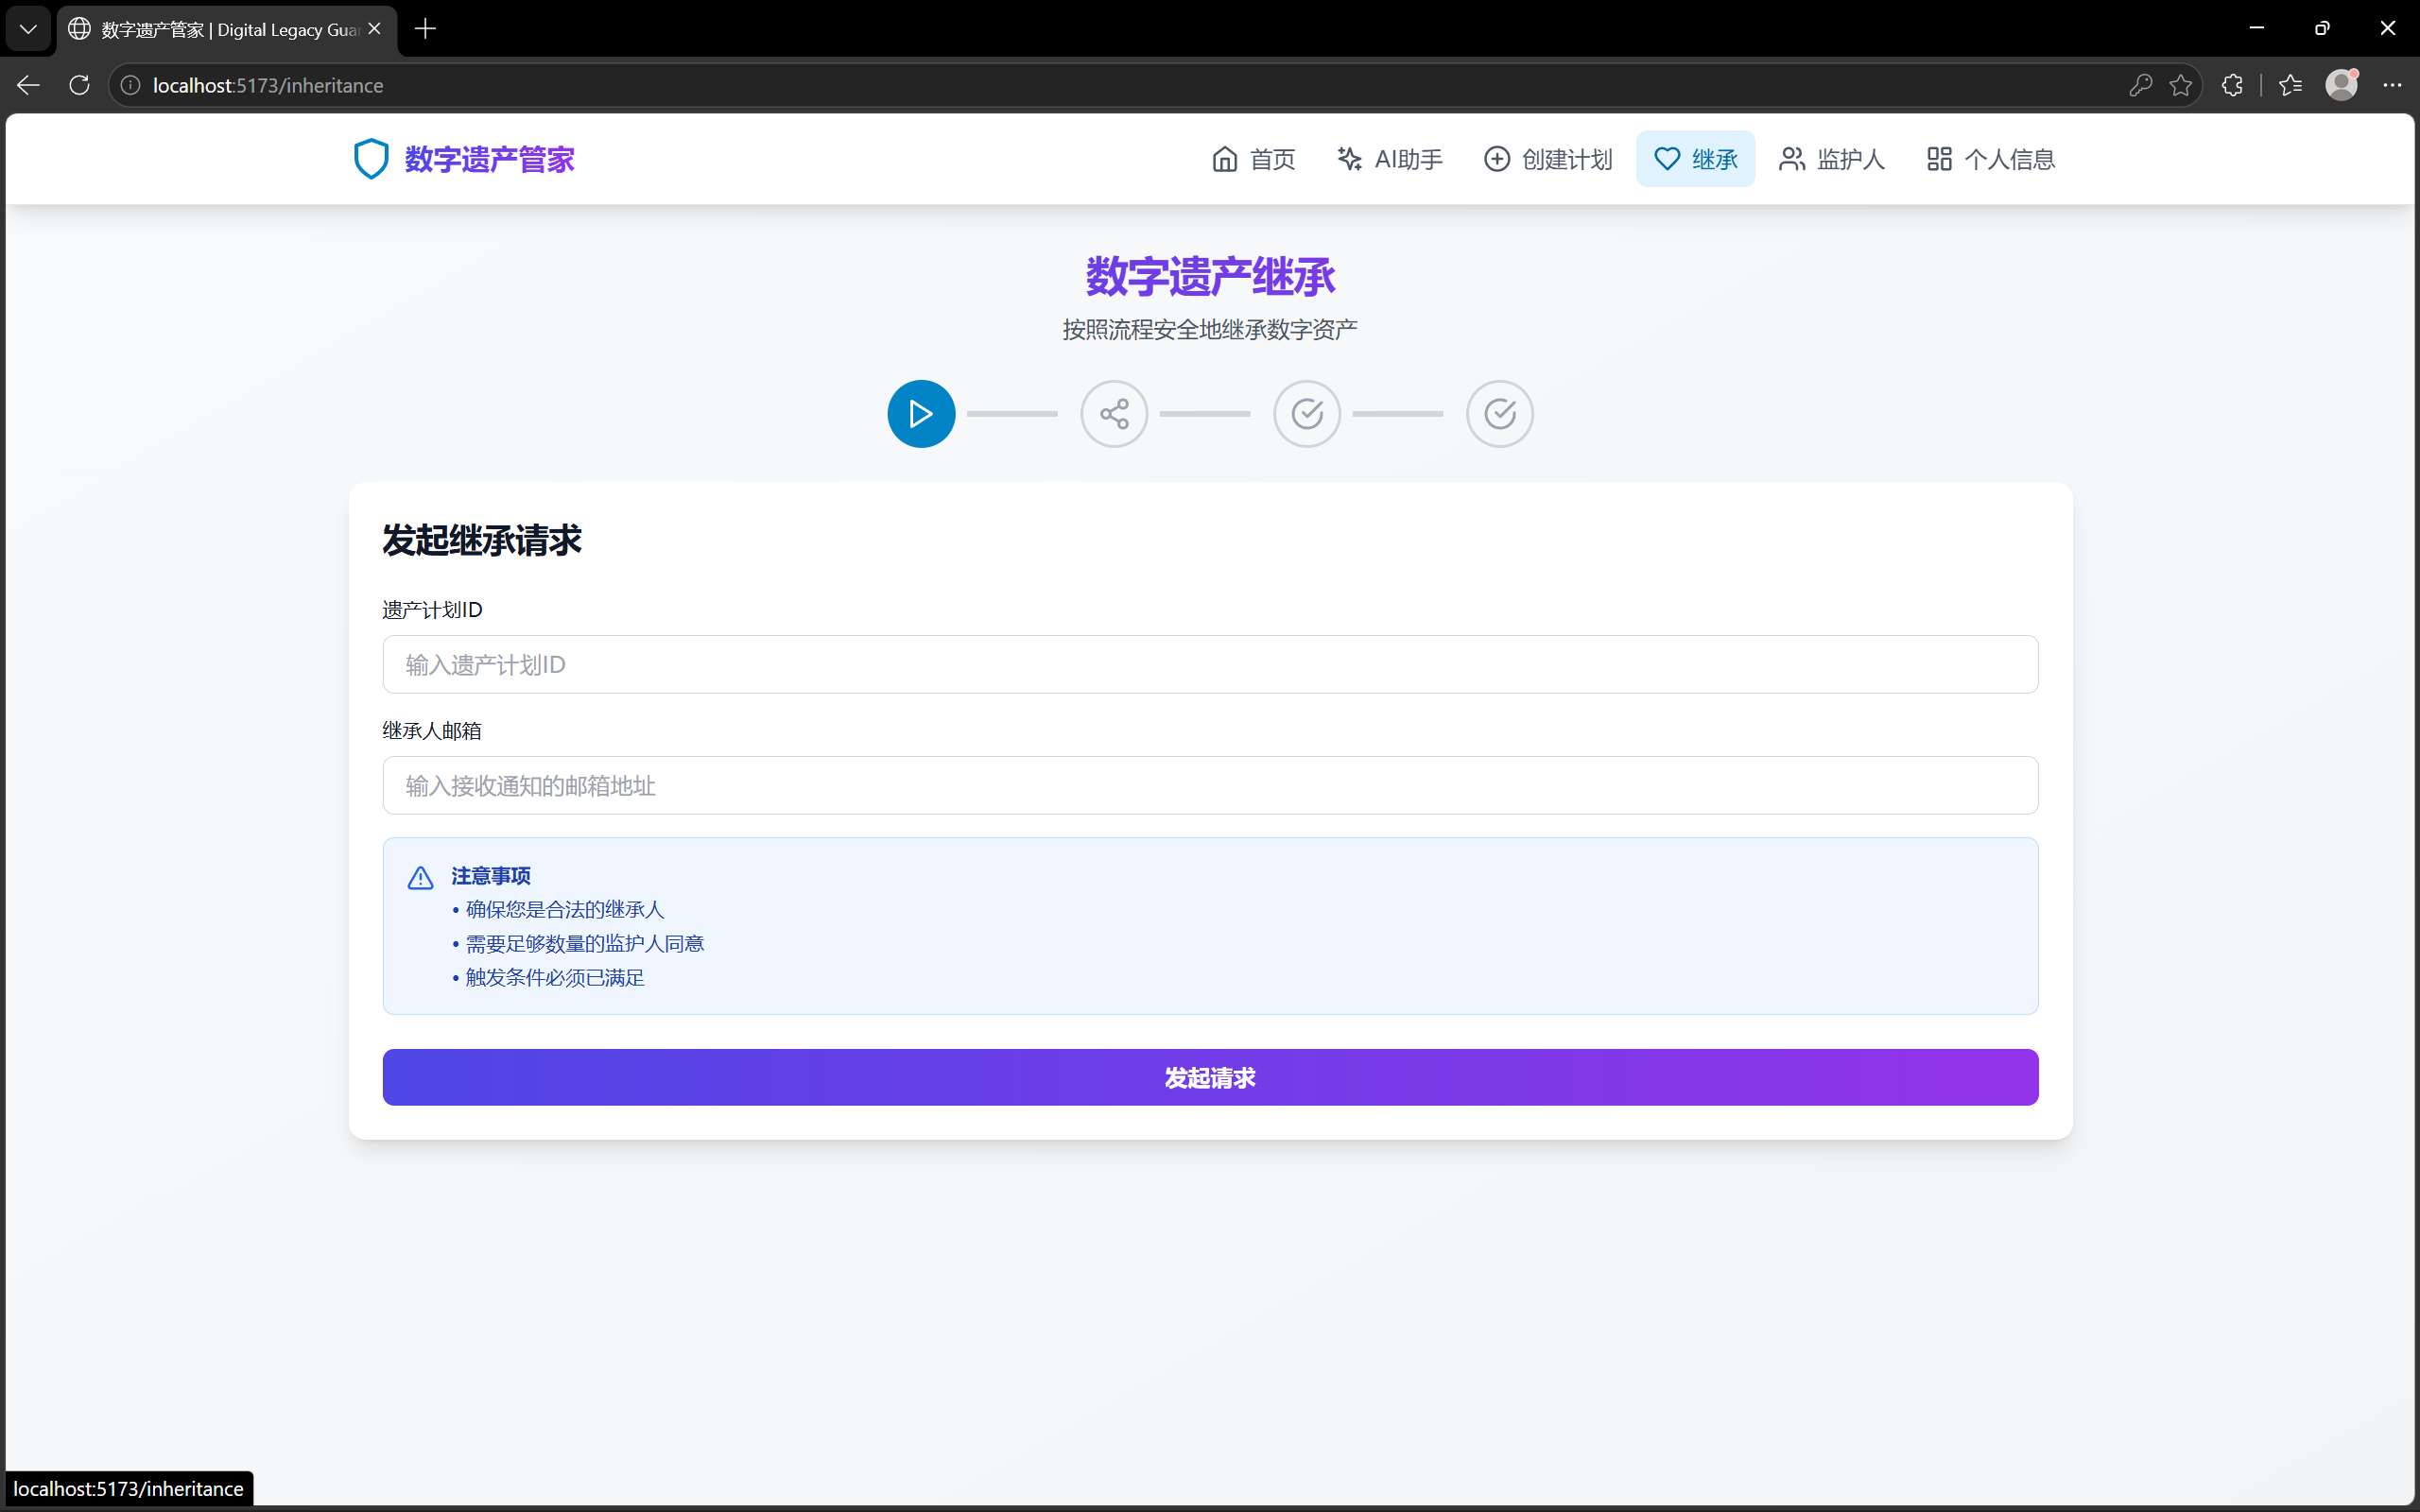
\includegraphics[width=1.0\textwidth]{figures/screenshots/继承发起页面.png}
\caption{继承发起页面——输入计划ID和继承人邮箱即可发起继承请求，后端自动检查时间锁并通知全体监护人}
\label{fig:ss_inherit}
\end{figure}

继承发起页面（图\ref{fig:ss_inherit}）将继承流程简化为"输入计划ID + 继承人邮箱"两步操作。后端在收到请求后自动执行时间锁检查（timed模式下精确计算剩余时间），通过后变更计划状态为collecting并向全体监护人发送邮件通知。若时间锁未到期，系统返回精确到秒的剩余时间信息。

\begin{figure}[H]
\centering
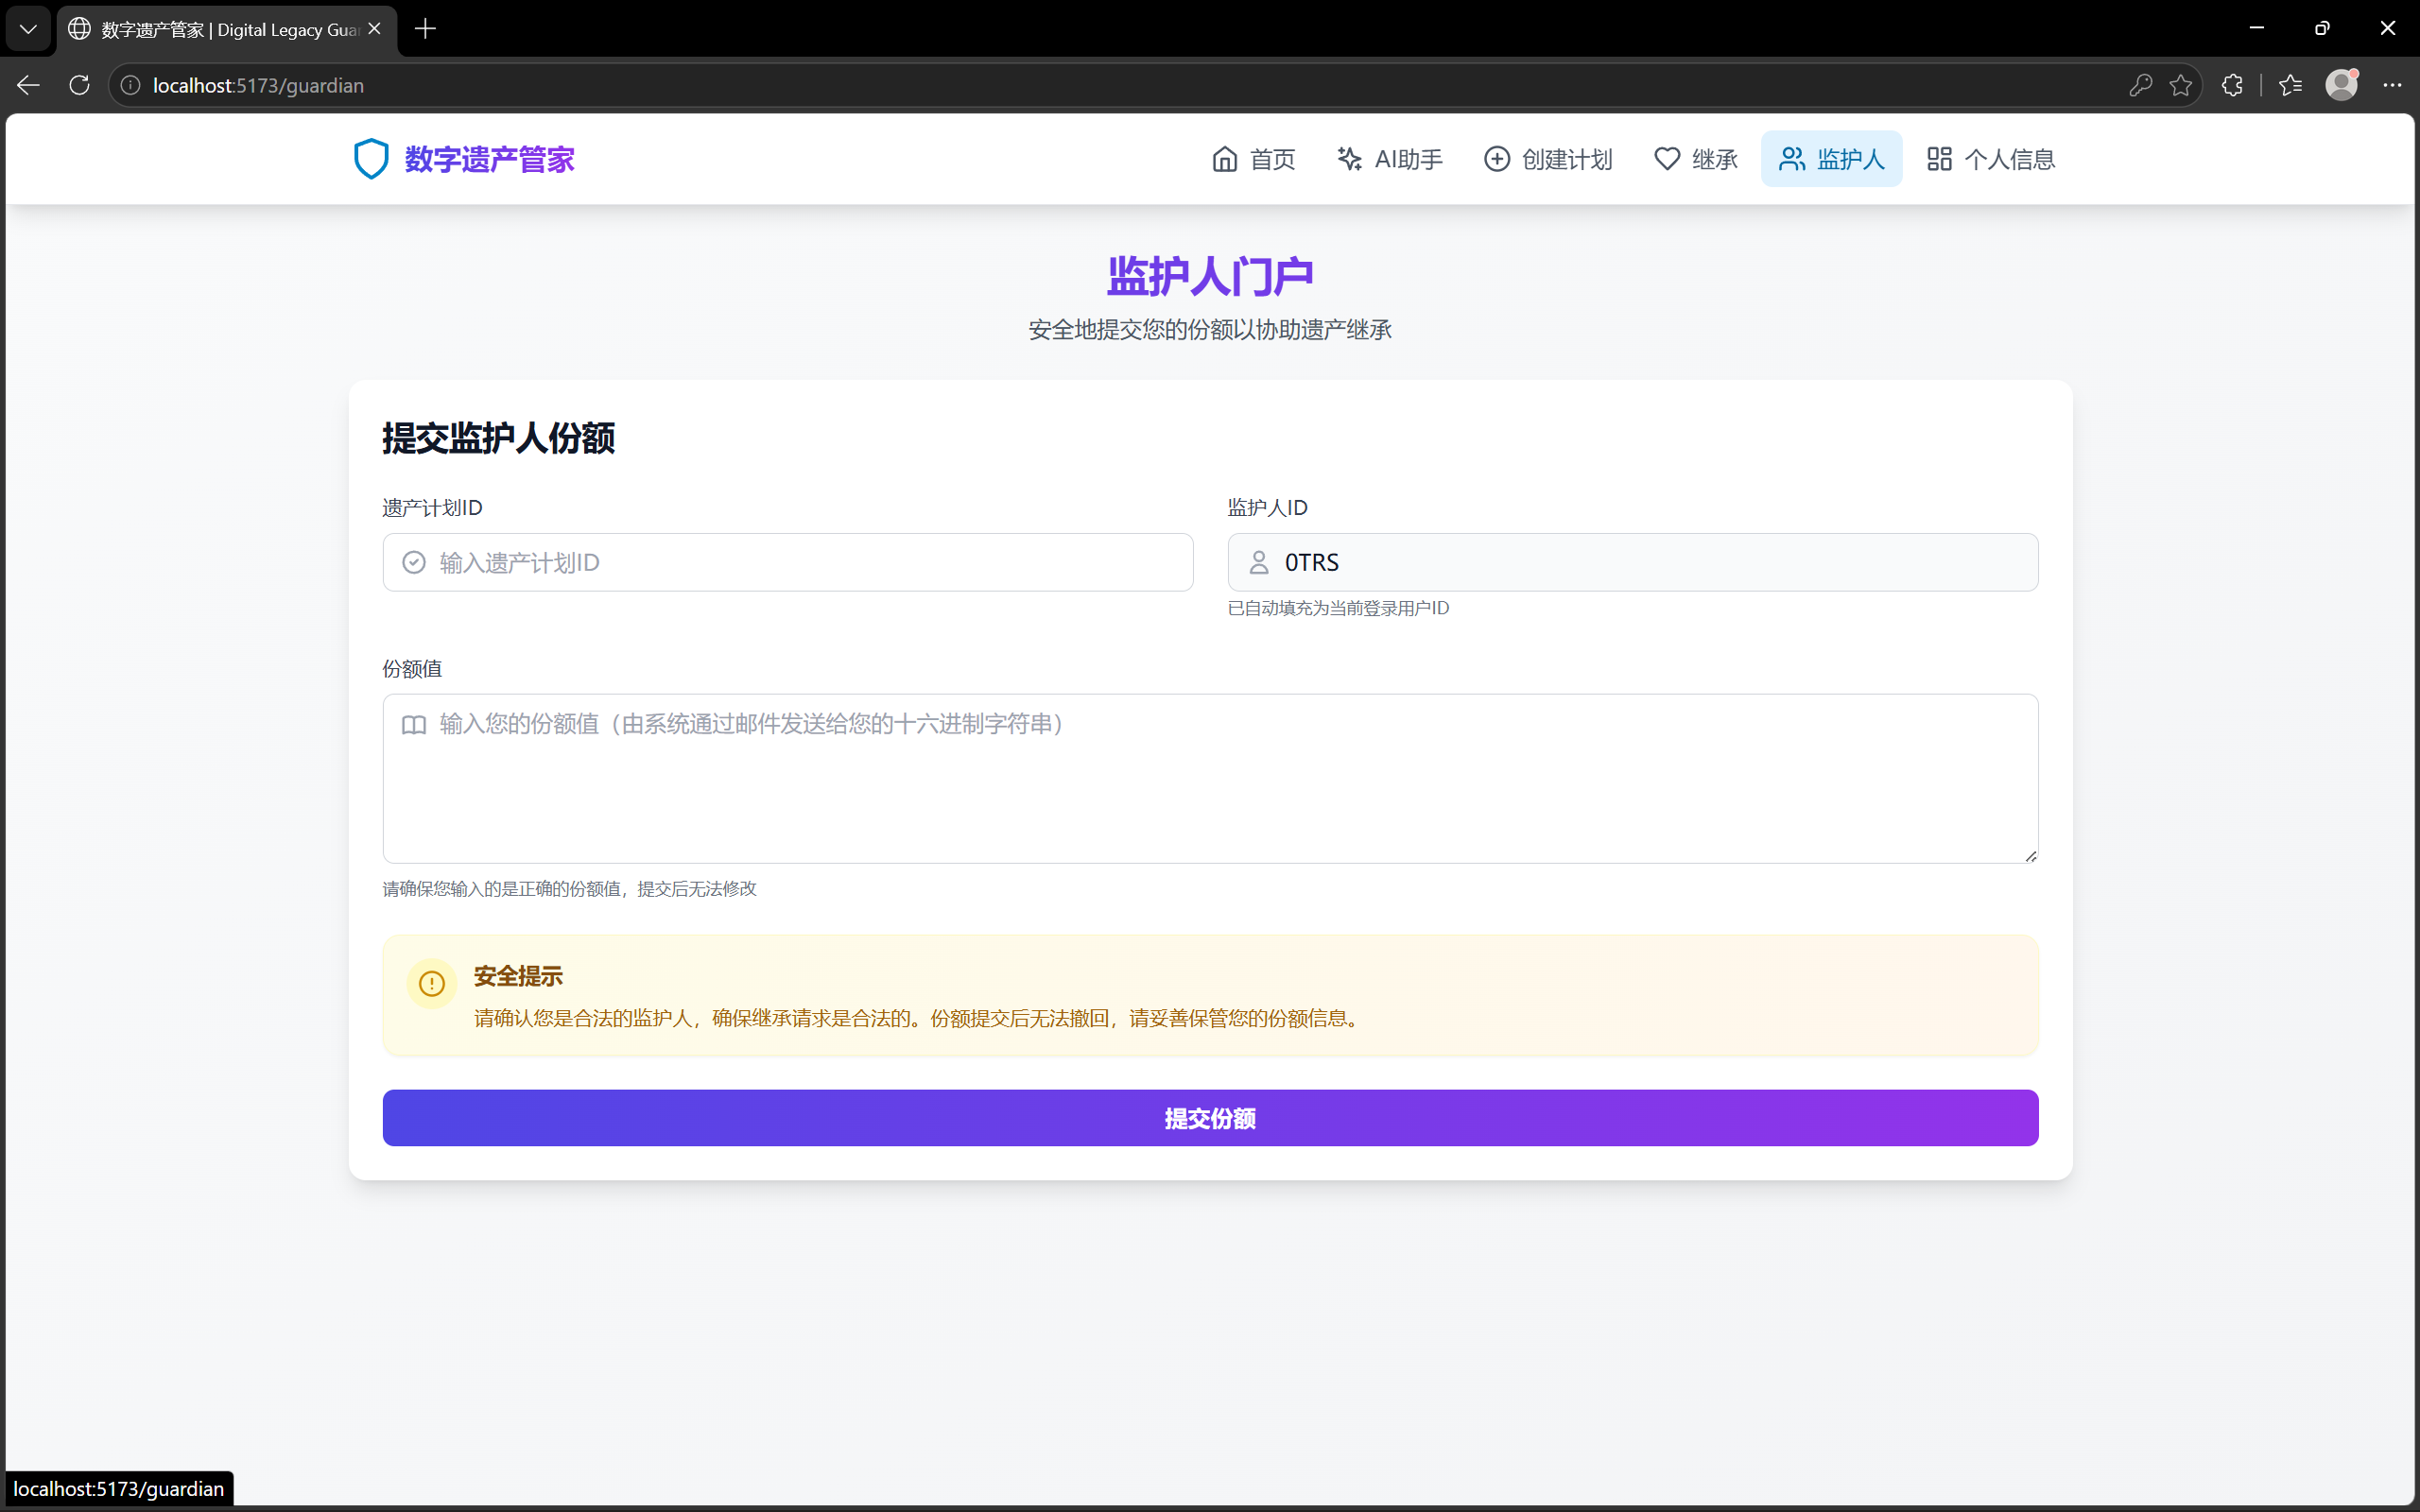
\includegraphics[width=1.0\textwidth]{figures/screenshots/监护人份额提交页面.png}
\caption{监护人份额提交页面——输入三项信息（计划ID、用户ID、份额值）即可提交，后端自动完成Pedersen单点验证和胁迫码检测}
\label{fig:ss_guardian}
\end{figure}

监护人份额提交页面（图\ref{fig:ss_guardian}）是监护人参与继承流程的唯一操作界面。监护人仅需输入计划ID、自身用户ID和邮件中收到的份额值（十六进制字符串）三项信息。后端在收到提交后自动执行份额值格式校验、Pedersen承诺匹配验证、胁迫码检测和防重复提交检查，监护人无需理解椭圆曲线密码学即可完成安全操作。

% ==================== 第四章 创新性说明 ====================
\chapter{创新性说明}

\section{场景创新：数字遗产全生命周期模型}

目前秘密共享、门限签名等密码学技术大多以密钥备份、企业容灾或区块链钱包恢复作为典型应用场景，研究重点通常集中于算法正确性和安全性验证。然而数字遗产继承场景同时涉及密码学、安全工程、法律规则以及社会关系管理等多个维度，其复杂程度远高于传统密钥备份问题。

本作品将门限密码学应用于数字遗产继承领域，构建了从资产托管、继承触发到秘密恢复的完整业务闭环。与传统密码保险箱不同，本系统不仅关注秘密的保存，更关注秘密在未来特定条件下的安全释放。系统需要同时解决“提前泄露风险”和“永久丢失风险”之间的矛盾——资产既不能在继承前被非法获取，也不能因持有人失联而永久不可访问。

具体而言，本作品将数字遗产继承抽象为五个有序阶段：\textbf{资产托管}（加密存储）$\to$ \textbf{条件触发}（时间或共识）$\to$ \textbf{份额验证}（双层密码学验证）$\to$ \textbf{密钥恢复}（拉格朗日插值）$\to$ \textbf{资产释放}（AES解密交付）。每个阶段均有明确的输入约束和输出保证，构成了一个可审计、可复现的安全流程。

此外，本作品支持加密货币私钥、数字版权文件、云存储账号以及智能合约权限等多种数字资产类型，使门限密码学从理论验证走向实际业务应用，具有较强的现实意义和推广价值。

\section{技术创新：双层可验证秘密共享机制}

在技术实现层面，本作品的核心创新在于通过 Pedersen 同态承诺构建了双层可验证秘密共享机制，使得份额的真实性能够在恢复操作之前以密码学强度得到验证。

传统秘密共享方案通常只保存份额数据本身，缺乏密码学强度的份额验证机制。当攻击者伪造份额或监护人提交错误数据时，系统往往只能在恢复阶段（即成功收集到足够份额后尝试恢复秘密时）才能发现问题。这种”恢复后发现错误”的模式存在严重缺陷：如果错误份额参与了拉格朗日插值，恢复出的秘密将是错误的；如果错误份额数量足够多，可能永远无法找到正确的份额组合。

本作品针对这一问题，设计了”恢复前验证”的安全模式：
\begin{enumerate}
  \item \textbf{第一层——Pedersen 单点承诺验证：}利用双多项式结构为每个份额生成 Pedersen 承诺 $C_i = r_iG + v_iH$，其中盲因子 $r_i$ 和份额值 $v_i$ 分别来自两个独立的 Shamir 多项式。提交份额时利用存储的盲因子重算承诺并比对，利用承诺的计算绑定性阻止份额值篡改。同时集成胁迫码检测——每位监护人持有正常份额和胁迫份额两组值，提交胁迫份额时系统触发警报并终止继承。
  \item \textbf{第二层——主承诺同态聚合验证：}创建时生成主承诺 $C_{\text{master}} = RG + sH$ 公开存储。恢复阶段利用 Lagrange 插值系数 $\lambda_i$ 和 Pedersen 承诺的同态性质，在椭圆曲线上直接验证 $\sum \lambda_i C_i \stackrel{?}{=} C_{\text{master}}$。这一层确保达到门限的 $t$ 个份额确实来源于同一个秘密共享实例，阻止跨计划份额注入攻击。
\end{enumerate}

两层机制在普通Web应用原型中实现了密码学强度的份额验证。实验表明，即使攻击者仅修改份额值中的一个十六进制字符，验证流程也能够在第一层准确识别异常并拒绝恢复请求。

\section{工程创新：全栈安全工程实践}

与多数密码学课程实验仅展示算法运行结果不同，本作品采用完整的全栈工程架构实现，从用户界面到密码学模块均具备独立运行和测试能力。

在系统架构设计上，本作品将密码学模块（crypto/shamir.ts）、业务逻辑模块（services/legacyPlanService.ts）、用户管理模块（services/userService.ts）、AI服务模块（services/aiService.ts）、邮件服务模块（services/emailService.ts）和展示模块（React前端）进行解耦，实现较好的模块化设计。密码学组件不依赖Express、不依赖文件系统、不依赖任何业务逻辑——它可以被独立引入、独立测试，并迁移到密钥托管、企业容灾恢复等其他安全系统中。

项目同时提供完整的需求分析、系统设计、测试验证和安全分析文档，使系统不仅能够运行，而且具备较好的可复现性和可审计性，更符合实际安全产品开发流程。

在可用性工程方面，本作品设计了多步骤创建向导和自然语言AI助手两种交互模式，降低了非专业用户配置Shamir参数（$t$和$n$）的学习门槛。监护人操作被精简为“输入三个字段+点击提交”的极简流程，不需要理解椭圆曲线密码学。

\section{可扩展性创新}

为了保证系统具备长期演进能力，本作品在架构设计阶段预留了多种扩展接口和升级路径。

在区块链层面，当前系统采用智能合约描述继承状态管理逻辑，合约中的createPlan和submitShare函数接受bytes32类型的承诺值，与后端的椭圆曲线承诺（压缩编码为33字节的十六进制字符串）兼容。未来可将完整的 Pedersen 同态承诺材料也提交至链上，实现完全去中心化的份额验证。

在存储层面，系统当前支持本地JSON文件存储，后续可通过将encryptedAssets字段迁移至IPFS或Arweave等去中心化存储网络（仅在数据库中保存内容标识符CID），实现遗产数据的长期不可篡改保存。

在业务层面，系统预留了短信通知、多因素认证、数字身份认证以及法律公证接口等扩展点。邮件服务的接口设计（emailService.sendXxx方法）不依赖特定的邮件基础设施，可替换为任何支持SMTP或API方式的服务提供商。

在密码学层面，系统当前使用secp256k1椭圆曲线（与比特币和以太坊兼容），但EC抽象层的设计（elliptic库的使用方式）使得切换到其他曲线（如ed25519或BLS12-381）成为可能，仅需更换EC构造函数参数和调整域参数。

在智能化方向，当前AI助手已支持基于 Deepseek 大模型的自然语言交互（见 §2.9），未来可进一步扩展至遗产配置建议、风险评估、继承规则自动生成以及异常行为检测等高级功能。

\section{与现有方案的详细对比}

为了更清晰地展现本作品的创新价值，以下从八个维度将本作品与现有典型方案进行系统对比。

\textbf{隐私保护。}传统遗嘱公证要求持有人将密码或助记词写入法律文书并由公证机构保管，公证人可直接查看敏感信息；中心化托管平台掌握用户资产全貌，存在内部人员作恶风险；链上多签钱包虽然通过智能合约分散控制权，但交易历史和签名方地址公开可见，缺乏隐私性；硬件恢复服务需要将身份信息提交给设备厂商完成KYC认证。相比之下，本作品将主密钥通过Shamir门限拆分为多个份额后分发给不同监护人，服务端仅存储Pedersen承诺值（$C_i = r_iG + v_iH$）而不保存份额明文，攻击者即便读取服务器全部数据也无法恢复主密钥或解密资产，在隐私保护维度上具有显著优势。

\textbf{抗单点失效。}传统遗嘱公证依赖单一公证机构，机构倒闭或内部人员变动即导致遗嘱无法执行；中心化托管将恢复能力完全寄托于平台持续运营，平台停服或被收购后资产面临风险；硬件恢复服务依赖厂商的长期存续和信誉。链上多签钱包通过智能合约实现了较好的去中心化，但守卫者丢失签名密钥同样是现实风险。本作品采用$t$-of-$n$门限恢复模型，只要任意$t$位监护人保持在线且诚实，即可完成资产恢复——部分监护人失联、拒绝配合甚至恶意作恶均不影响恢复流程，从根本上消除了单点失效风险。

\textbf{份额可验证。}传统遗嘱公证和中心化托管均不具备密码学强度的份额验证机制——公证处仅核验文书签章真实性，平台仅依赖账号密码认证，无法验证份额数据是否在传输或存储中被篡改。链上多签钱包的签名验证仅确认签名格式合法，不验证签名对应的份额是否来源于正确的秘密共享多项式。本作品构建了双层密码学验证机制：第一层 Pedersen 单点承诺验证（$C_i = r_iG + v_iH$）在提交时即阻止份额值篡改，同时集成胁迫码检测；第二层主承诺同态聚合验证（$\sum \lambda_i C_i \stackrel{?}{=} C_{\text{master}}$）确保份额集合来源于正确的秘密共享实例。两层验证在恢复操作执行前即可以密码学强度判定份额真实性，而非依赖"恢复后才发现错误"的脆弱模式。

\textbf{资产覆盖面。}传统遗嘱公证虽然理论上可覆盖所有类型财产，但数字资产（私钥、密码、Token URI）难以在文书中以机器可处理的形式精确表达；中心化托管仅覆盖特定平台内的资产（如交易所账户余额）；链上多签钱包仅管理EVM兼容链上的代币和合约权限；硬件恢复服务仅恢复特定硬件钱包中的密钥。本作品将加密货币私钥、云存储账号凭证、加密文件和智能合约权限统一抽象为资产类型，以同一套门限密码学协议进行托管，并提供可扩展的资产元数据结构，覆盖范围显著更广。

\textbf{触发灵活性。}传统遗嘱的触发完全依赖法律流程——遗嘱执行人申请、法院裁定、资产过户——周期漫长且缺乏自动化能力；中心化平台的触发条件由平台单方制定（如Google非活跃账户管理器仅支持固定非活跃期限），用户无法自定义；硬件恢复服务通常不提供触发条件配置。链上多签钱包支持自定义多签逻辑，但触发仅限于链上交易签名收集。本作品同时支持社会共识模式（任意$t$位监护人确认即可触发）和时间锁模式（指定天数后自动触发），智能合约进一步提供二者结合的混合模式，充分适应不同场景的触发需求。

\textbf{使用门槛。}传统遗嘱公证需要经历律师咨询、文书起草、公证员见证等法律流程，时间成本和费用均较高；链上多签钱包需要理解Gas费、合约交互、签名构造等区块链概念，对普通用户极不友好。中心化托管的用户体验较好（通常为平台内置功能），硬件恢复服务也提供引导式操作。本作品在前端设计了四步向导式创建流程（资产配置 $\to$ 监护人设置 $\to$ 触发条件 $\to$ 确认创建），每步包含实时表单验证和中文提示，同时提供AI助手通过自然语言对话引导用户完成操作，监护人仅需输入三个字段即可提交份额，将门限密码学的专业配置门槛降至最低。

\textbf{去中心化。}传统遗嘱公证、中心化托管和硬件恢复服务均为中心化架构，依赖单一机构或厂商作为信任锚点。链上多签钱包通过智能合约实现了高度的去中心化——资金由合约代码而非任何个人控制。本作品在服务端架构层面仍为客户端-服务器模型，但密码学安全不依赖服务器的可信性——服务器不持有主密钥和份额明文，仅作为公开承诺值和加密资产的存储中介。智能合约可选部署至以太坊兼容链，将计划元数据、监护人承诺映射和状态转换逻辑交由链上合约管理，实现从"信任服务器"到"信任数学与共识"的逐步过渡。

\textbf{可审计性。}传统遗嘱公证的法律文书具有天然的审计属性，但审计范围仅限于文书签署和保管过程，无法追踪数字资产的后续流转；中心化托管平台通常不向用户提供完整的操作日志；链上多签钱包的所有交易和签名均在链上公开记录，审计性最强。本作品在服务端记录计划创建、继承申请、份额提交、密钥恢复等全生命周期事件（含时间戳、操作者身份和操作结果），同时智能合约通过indexed事件（PlanCreated、ShareSubmitted、PlanTriggered、PlanCompleted）在链上提供不可篡改的审计轨迹，兼顾了线下审计的完整性和链上审计的不可抵赖性。

综上所述，本作品在隐私保护、抗单点失效、份额可验证性、资产覆盖面和触发灵活性五个维度上全面领先现有方案，在使用门槛维度上接近最优水平，并在去中心化和可审计性上与链上方案形成互补。

\section{工程实现的创新价值}

本作品的工程实现本身也构成创新贡献。当前多数密码学课程实验停留在命令行或Jupyter Notebook层面的算法演示，缺乏完整的交互界面、错误处理和生命周期管理。本作品将 Shamir 秘密共享、Pedersen 同态承诺和同态份额刷新三项密码学技术集成到一个具有生产级代码质量的全栈 Web 应用中，证明了这些技术在真实网络环境中的可行性。

具体而言，密码学模块的设计遵循以下工程原则：一是\textbf{接口隔离}——ShamirSecretSharing 接口定义清晰的 split/combine/verify 方法签名，调用方无需了解有限域运算或椭圆曲线细节；二是\textbf{安全默认}——构造函数自动校验域阶与群阶一致性，防止错误域参数导致密码学失效；三是\textbf{类型安全}——TypeScript 严格模式覆盖密码学模块，所有椭圆曲线运算和模逆运算有 try-catch 保护，模块无文件系统依赖，满足纯函数设计原则。

这些工程实践使得密码学模块可以被其他项目直接复用。例如，一个企业密钥托管系统可以引入 shamir.ts 而无需修改任何代码，仅需按照接口契约提供参数即可实现密钥的门限拆分和可验证恢复。

\section{社会价值与应用前景展望}

数字遗产问题不仅是一个技术问题，更是一个日益紧迫的社会问题。根据统计，全球因私钥丢失而永久无法访问的比特币已超过 370 万枚（价值超过 1000 亿美元）。随着 Web3、DeFi 和 NFT 的普及，越来越多的个人财富以纯数字形式存在，而相应的继承基础设施严重滞后。本作品的技术方案为社会提供了一个可行的解决路径：通过门限密码学将“单人掌握密钥”转化为“多人协作恢复”，在隐私保护和继承可达性之间取得了工程平衡。

在应用前景方面，本作品可向以下方向演进：与法律科技（LegalTech）公司合作，将数字遗产计划与法律遗嘱签署流程整合；与加密货币交易所和钱包服务商合作，作为其“遗产托管”功能的开源参考实现；与云服务商（如 AWS KMS、Google Cloud KMS）集成，利用硬件安全模块保护份额分发过程；扩展到去中心化身份（DID）和可验证凭证（VC）领域，实现数字身份的跨代传递。

% ==================== 第五章 总结 ====================
\chapter{总结}

\section{工作总结}

本作品\project（\englishname）围绕数字资产继承中的单点失效、隐私泄露、提前释放和伪造份额四大核心问题，完成了一个从理论到实现的全栈可运行原型系统。系统将Shamir秘密共享、Pedersen同态承诺、AES对称加密、ECIES份额传输加密、REST API服务、React前端向导、Solidity智能合约状态机和自然语言AI助手等多项技术有机结合起来，实现了从资产托管到继承恢复的完整安全闭环。

在密码学层面，本作品在普通Web应用原型中成功落地了可验证秘密共享机制。双层验证机制——Pedersen单点承诺验证和主承诺同态聚合验证——确保份额的真实性可以在恢复操作之前得到密码学强度的验证，而非依赖”恢复后才发现错误”的脆弱模式。同态份额刷新（零和多项式方法）实现在不接触主密钥的前提下安全轮换所有份额及其承诺。

在安全工程层面，本作品贯彻了“最小化存储敏感数据”的原则。StoredShare与Share的差分设计使得持久化存储中不含份额明文值；主密钥仅在创建时的局部变量中存在，拆分后即被丢弃；加密资产包的密钥本身也通过门限拆分保护。这些设计确保了即使攻击者获得服务器文件系统的完全读取权限，也无法直接获取资产内容。

在架构层面，本作品实现了密码学模块、业务逻辑模块、数据管理模块和展示模块的解耦设计。密码学模块可独立测试和迁移复用，业务服务关注生命周期管理而不涉及底层密码学细节，前端提供可视化的多步骤向导降低用户使用门槛。智能合约表达了去中心化条件下的状态约束和触发条件，为未来的链上部署提供了清晰的接口规范。

本报告依据竞赛要求编写，保留摘要、作品概述、设计与实现、测试与分析、创新性说明、总结和参考文献的标准结构，补充了大量架构图、流程图、状态图、表格和代码片段。报告避免出现学校、院系、指导教师等身份信息，满足网评匿名性要求。

\section{不足与展望}

当前系统仍属于竞赛原型阶段，在迈向生产级部署的过程中还存在以下不足：

\begin{enumerate}
  \item \textbf{持久化方案简化：}当前使用本地JSON文件存储，缺少事务支持、并发控制和故障恢复能力。生产环境应将plans和requests迁移至PostgreSQL关系数据库，将encryptedAssets字段迁移至IPFS或AWS S3对象存储（数据库中仅保存CID或对象键）。
  \item \textbf{份额分发渠道单一：}当前份额仅通过电子邮件发送给监护人。虽然SMTP通常运行在TLS之上，但邮件服务提供商可以读取邮件内容。未来可引入端到端加密（使用监护人的公钥加密份额）、安全消息应用（如Signal）或硬件安全模块（HSM）作为额外的份额分发渠道。
  \item \textbf{智能合约仅本地测试：}当前合约在Hardhat本地网络测试，尚未部署到任何公共测试网或主网。未来的工作包括：将合约部署至以太坊Sepolia测试网或Layer 2网络（如Polygon、Arbitrum）；引入门限签名（如BLS门限签名）实现在链上聚合签名以完成资产转移；将Pedersen同态承诺材料的哈希提交至链上，实现链上可验证的份额提交。
  \item \textbf{性能未充分压测：}当前原型仅在单一开发者机器上进行功能验证，未进行并发压力测试和性能基准测试。生产环境需评估在数百个并发计划下的JSON文件读写性能，以及门限参数较大（如50-of-100）时的多项式运算性能。
  \item \textbf{身份认证与授权不完整：}当前缺少JWT令牌机制或OAuth集成，API请求未携带认证令牌（仅通过请求参数传递userId）。生产环境应在登录后签发JWT，在API网关层进行令牌验证。
  \item \textbf{零知识份额验证：}当前份额验证基于 Pedersen 单点承诺——服务端利用存储的盲因子 $r_i$ 重算承诺以验证份额值，这要求服务端持有盲因子，属于"不受信第三方"模型。后续迭代中计划引入非份额提交模式下的份额验证功能，该功能可以基于由schnorr数字签名实现交互式零知识证明，支持在不向server暴露可能份额值的前提下，验证当前份额的有效性，具有现实的密码学意义
  \item \textbf{生命体征监测系统触发机制：}当前触发机制基于社会共识，或者事件锁机制，只能粗略的预测遗产持有人的失能时间，后续项目迭代中，计划引入生命体征检测系统和server的通信机制，实现基于硬件生命体征监测机制的触发模式。当前受制于硬件实现困难，暂时难以部署相关功能，但该迭代方向具有重大现实意义。
  \item \textbf{AI助手功能有待完善：}当前 AI 助手已支持基于 Deepseek 大模型的自然语言交互，但工具调用范围局限于创建计划、继承请求、份额提交和状态查询等基础操作。未来可扩展至遗产配置建议、风险评估、继承规则自动生成以及异常行为检测等高级功能。
\end{enumerate}

尽管存在上述不足，本作品在当前竞赛原型阶段已经实现了一个功能完整、密码学机制正确、安全设计合理的数字遗产继承系统。系统各模块的接口清晰、代码可读性良好、测试覆盖充分，为后续的工程化迭代和学术研究提供了扎实的基础。

% ==================== 参考文献 ====================
\chapter*{参考文献}
\addcontentsline{toc}{chapter}{参考文献}

[1] Shamir A. How to share a secret[J]. Communications of the ACM, 1979, 22(11): 612-613.

[2] Feldman P. A practical scheme for non-interactive verifiable secret sharing[C]//Proceedings of the 28th Annual Symposium on Foundations of Computer Science. IEEE, 1987: 427-438.

[3] Schnorr C P. Efficient signature generation by smart cards[J]. Journal of Cryptology, 1991, 4(3): 161-174.

[4] Nakamoto S. Bitcoin: A peer-to-peer electronic cash system[EB/OL]. 2008.

[5] Wood G. Ethereum: A secure decentralised generalised transaction ledger[EB/OL]. 2014.

[6] Benaloh J. Secret sharing homomorphisms: Keeping shares of a secret secret[C]//Advances in Cryptology — CRYPTO '86. Springer, 1987: 251-260.

[7] Pedersen T P. Non-interactive and information-theoretic secure verifiable secret sharing[C]//Advances in Cryptology — CRYPTO '91. Springer, 1991: 129-140.

[8] National Institute of Standards and Technology. Digital Signature Standard (DSS), FIPS PUB 186-5[S]. 2023.

[9] National Institute of Standards and Technology. Recommendation for Block Cipher Modes of Operation, SP 800-38A[S]. 2001.

[10] National Institute of Standards and Technology. Recommendation for Password-Based Key Derivation, SP 800-132[S]. 2010.

[11] Bernstein D J, Duif N, Lange T, et al. High-speed high-security signatures[J]. Journal of Cryptographic Engineering, 2012, 2(2): 77-89.

[12] Fiat A, Shamir A. How to prove yourself: Practical solutions to identification and signature problems[C]//Advances in Cryptology — CRYPTO '86. Springer, 1987: 186-194.

[13] OpenZeppelin. Smart Contract Security Guidelines[EB/OL]. \url{https://docs.openzeppelin.com/}.

[14] Solidity Team. Solidity v0.8 Documentation[EB/OL]. \url{https://docs.soliditylang.org/}.

[15] Ethereum Foundation. Ethereum Yellow Paper[EB/OL]. 2024.

[16] Hardhat. Ethereum development environment documentation[EB/OL]. \url{https://hardhat.org/docs}.

[17] React Team. React v18 Documentation[EB/OL]. \url{https://react.dev/}.

[18] Express.js. Express 4.x API Reference[EB/OL]. \url{https://expressjs.com/}.

[19] TypeScript Team. TypeScript Handbook[EB/OL]. \url{https://www.typescriptlang.org/docs/}.

[20] elliptic. Fast Elliptic Curve Cryptography in plain JavaScript[EB/OL]. \url{https://github.com/indutny/elliptic}.

[21] CryptoJS. JavaScript library of crypto standards[EB/OL]. \url{https://github.com/brix/crypto-js}.

[22] GB/T 7714-2015. 信息与文献 参考文献著录规则[S]. 中国标准出版社, 2015.

[23] Merkle R C. A digital signature based on a conventional encryption function[C]//Advances in Cryptology — CRYPTO '87. Springer, 1987: 369-378.

[24] Bellare M, Rogaway P. Random oracles are practical: A paradigm for designing efficient protocols[C]//Proceedings of the 1st ACM Conference on Computer and Communications Security. 1993: 62-73.

[25] Menezes A J, Van Oorschot P C, Vanstone S A. Handbook of Applied Cryptography[M]. CRC Press, 1996.

\end{document}
